% Options for packages loaded elsewhere
\PassOptionsToPackage{unicode}{hyperref}
\PassOptionsToPackage{hyphens}{url}
\PassOptionsToPackage{dvipsnames,svgnames*,x11names*}{xcolor}
%
\documentclass[
]{krantz}
\usepackage{lmodern}
\usepackage{amssymb,amsmath}
\usepackage{ifxetex,ifluatex}
\ifnum 0\ifxetex 1\fi\ifluatex 1\fi=0 % if pdftex
  \usepackage[T1]{fontenc}
  \usepackage[utf8]{inputenc}
  \usepackage{textcomp} % provide euro and other symbols
\else % if luatex or xetex
  \usepackage{unicode-math}
  \defaultfontfeatures{Scale=MatchLowercase}
  \defaultfontfeatures[\rmfamily]{Ligatures=TeX,Scale=1}
\fi
% Use upquote if available, for straight quotes in verbatim environments
\IfFileExists{upquote.sty}{\usepackage{upquote}}{}
\IfFileExists{microtype.sty}{% use microtype if available
  \usepackage[]{microtype}
  \UseMicrotypeSet[protrusion]{basicmath} % disable protrusion for tt fonts
}{}
\makeatletter
\@ifundefined{KOMAClassName}{% if non-KOMA class
  \IfFileExists{parskip.sty}{%
    \usepackage{parskip}
  }{% else
    \setlength{\parindent}{0pt}
    \setlength{\parskip}{6pt plus 2pt minus 1pt}}
}{% if KOMA class
  \KOMAoptions{parskip=half}}
\makeatother
\usepackage{xcolor}
\IfFileExists{xurl.sty}{\usepackage{xurl}}{} % add URL line breaks if available
\IfFileExists{bookmark.sty}{\usepackage{bookmark}}{\usepackage{hyperref}}
\hypersetup{
  pdftitle={GLMs and Multilevel Models},
  pdfauthor={Paul Roback and Julie Legler},
  colorlinks=true,
  linkcolor=Maroon,
  filecolor=Maroon,
  citecolor=Blue,
  urlcolor=Blue,
  pdfcreator={LaTeX via pandoc}}
\urlstyle{same} % disable monospaced font for URLs
\usepackage{color}
\usepackage{fancyvrb}
\newcommand{\VerbBar}{|}
\newcommand{\VERB}{\Verb[commandchars=\\\{\}]}
\DefineVerbatimEnvironment{Highlighting}{Verbatim}{commandchars=\\\{\}}
% Add ',fontsize=\small' for more characters per line
\usepackage{framed}
\definecolor{shadecolor}{RGB}{248,248,248}
\newenvironment{Shaded}{\begin{snugshade}}{\end{snugshade}}
\newcommand{\AlertTok}[1]{\textcolor[rgb]{0.33,0.33,0.33}{#1}}
\newcommand{\AnnotationTok}[1]{\textcolor[rgb]{0.37,0.37,0.37}{\textbf{\textit{#1}}}}
\newcommand{\AttributeTok}[1]{\textcolor[rgb]{0.61,0.61,0.61}{#1}}
\newcommand{\BaseNTok}[1]{\textcolor[rgb]{0.06,0.06,0.06}{#1}}
\newcommand{\BuiltInTok}[1]{#1}
\newcommand{\CharTok}[1]{\textcolor[rgb]{0.5,0.5,0.5}{#1}}
\newcommand{\CommentTok}[1]{\textcolor[rgb]{0.37,0.37,0.37}{\textit{#1}}}
\newcommand{\CommentVarTok}[1]{\textcolor[rgb]{0.37,0.37,0.37}{\textbf{\textit{#1}}}}
\newcommand{\ConstantTok}[1]{\textcolor[rgb]{0,0,0}{#1}}
\newcommand{\ControlFlowTok}[1]{\textcolor[rgb]{0.27,0.27,0.27}{\textbf{#1}}}
\newcommand{\DataTypeTok}[1]{\textcolor[rgb]{0.27,0.27,0.27}{#1}}
\newcommand{\DecValTok}[1]{\textcolor[rgb]{0.06,0.06,0.06}{#1}}
\newcommand{\DocumentationTok}[1]{\textcolor[rgb]{0.37,0.37,0.37}{\textbf{\textit{#1}}}}
\newcommand{\ErrorTok}[1]{\textcolor[rgb]{0.14,0.14,0.14}{\textbf{#1}}}
\newcommand{\ExtensionTok}[1]{#1}
\newcommand{\FloatTok}[1]{\textcolor[rgb]{0.06,0.06,0.06}{#1}}
\newcommand{\FunctionTok}[1]{\textcolor[rgb]{0,0,0}{#1}}
\newcommand{\ImportTok}[1]{#1}
\newcommand{\InformationTok}[1]{\textcolor[rgb]{0.37,0.37,0.37}{\textbf{\textit{#1}}}}
\newcommand{\KeywordTok}[1]{\textcolor[rgb]{0.27,0.27,0.27}{\textbf{#1}}}
\newcommand{\NormalTok}[1]{#1}
\newcommand{\OperatorTok}[1]{\textcolor[rgb]{0.43,0.43,0.43}{\textbf{#1}}}
\newcommand{\OtherTok}[1]{\textcolor[rgb]{0.37,0.37,0.37}{#1}}
\newcommand{\PreprocessorTok}[1]{\textcolor[rgb]{0.37,0.37,0.37}{\textit{#1}}}
\newcommand{\RegionMarkerTok}[1]{#1}
\newcommand{\SpecialCharTok}[1]{\textcolor[rgb]{0,0,0}{#1}}
\newcommand{\SpecialStringTok}[1]{\textcolor[rgb]{0.5,0.5,0.5}{#1}}
\newcommand{\StringTok}[1]{\textcolor[rgb]{0.5,0.5,0.5}{#1}}
\newcommand{\VariableTok}[1]{\textcolor[rgb]{0,0,0}{#1}}
\newcommand{\VerbatimStringTok}[1]{\textcolor[rgb]{0.5,0.5,0.5}{#1}}
\newcommand{\WarningTok}[1]{\textcolor[rgb]{0.37,0.37,0.37}{\textbf{\textit{#1}}}}
\usepackage{longtable,booktabs}
% Correct order of tables after \paragraph or \subparagraph
\usepackage{etoolbox}
\makeatletter
\patchcmd\longtable{\par}{\if@noskipsec\mbox{}\fi\par}{}{}
\makeatother
% Allow footnotes in longtable head/foot
\IfFileExists{footnotehyper.sty}{\usepackage{footnotehyper}}{\usepackage{footnote}}
\makesavenoteenv{longtable}
\usepackage{graphicx,grffile}
\makeatletter
\def\maxwidth{\ifdim\Gin@nat@width>\linewidth\linewidth\else\Gin@nat@width\fi}
\def\maxheight{\ifdim\Gin@nat@height>\textheight\textheight\else\Gin@nat@height\fi}
\makeatother
% Scale images if necessary, so that they will not overflow the page
% margins by default, and it is still possible to overwrite the defaults
% using explicit options in \includegraphics[width, height, ...]{}
\setkeys{Gin}{width=\maxwidth,height=\maxheight,keepaspectratio}
% Set default figure placement to htbp
\makeatletter
\def\fps@figure{htbp}
\makeatother
\setlength{\emergencystretch}{3em} % prevent overfull lines
\providecommand{\tightlist}{%
  \setlength{\itemsep}{0pt}\setlength{\parskip}{0pt}}
\setcounter{secnumdepth}{5}
\usepackage{booktabs}
%These packages added to resolve tex problems arising from kable tables.
\usepackage{tabularx}
\usepackage{float}
%%
\usepackage{longtable}
\usepackage[bf,singlelinecheck=off]{caption}

\usepackage{framed,color}
\definecolor{shadecolor}{RGB}{248,248,248}

\renewcommand{\textfraction}{0.05}
\renewcommand{\topfraction}{0.8}
\renewcommand{\bottomfraction}{0.8}
\renewcommand{\floatpagefraction}{0.75}

%%%%%%%%
% Inserting new commands here

%% Chapter 2
\newcommand{\lik}{\mathrm{Lik}}
\newcommand{\Lik}{\mathrm{Lik}}

\newcommand{\bstop}{p_{S|B1}}
\newcommand{\nstop}{p_{S|N}}

\newcommand{\thisismynewcommand}{p_{B|\textrm{B Bias}}}
\newcommand{\neutral}{p_{B|N}}
\newcommand{\gbias}{p_{B|\textrm{G Bias}}}
\newcommand{\bbias}{p_{B|\textrm{B Bias}}}

%% Chapter 3
\newcommand{\E}{\operatorname{E}}
\newcommand{\SD}{\operatorname{SD}}

%% Chapter 5
\newcommand{\var}{\operatorname{Var}}

%%%%%%%%

\renewenvironment{quote}{\begin{VF}}{\end{VF}}
\let\oldhref\href
\renewcommand{\href}[2]{#2\footnote{\url{#1}}}

\makeatletter
\newenvironment{kframe}{%
\medskip{}
\setlength{\fboxsep}{.8em}
 \def\at@end@of@kframe{}%
 \ifinner\ifhmode%
  \def\at@end@of@kframe{\end{minipage}}%
  \begin{minipage}{\columnwidth}%
 \fi\fi%
 \def\FrameCommand##1{\hskip\@totalleftmargin \hskip-\fboxsep
 \colorbox{shadecolor}{##1}\hskip-\fboxsep
     % There is no \\@totalrightmargin, so:
     \hskip-\linewidth \hskip-\@totalleftmargin \hskip\columnwidth}%
 \MakeFramed {\advance\hsize-\width
   \@totalleftmargin\z@ \linewidth\hsize
   \@setminipage}}%
 {\par\unskip\endMakeFramed%
 \at@end@of@kframe}
\makeatother

% This change to the shaded environment adapted from https://github.com/yihui/bookdown-chinese/commit/a3e392593b464ba31a7eceb0cd60f7e0bd112798 and https://stackoverflow.com/questions/41052687/rstudio-pdf-knit-fails-with-environment-shaded-undefined-error
\makeatletter
\@ifundefined{Shaded}{
}{\renewenvironment{Shaded}{\begin{kframe}}{\end{kframe}}}
\makeatother

\usepackage{makeidx}
\makeindex

\urlstyle{tt}

\usepackage{amsthm}
\makeatletter
\def\thm@space@setup{%
  \thm@preskip=8pt plus 2pt minus 4pt
  \thm@postskip=\thm@preskip
}
\makeatother

\frontmatter
\usepackage[]{natbib}
\bibliographystyle{plainnat}

\title{GLMs and Multilevel Models}
\usepackage{etoolbox}
\makeatletter
\providecommand{\subtitle}[1]{% add subtitle to \maketitle
  \apptocmd{\@title}{\par {\large #1 \par}}{}{}
}
\makeatother
\subtitle{Broadening Your Statistical Horizons with Applications using R}
\author{Paul Roback and Julie Legler}
\date{2020-06-26}

\begin{document}
\maketitle

% you may need to leave a few empty pages before the dedication page

%\cleardoublepage\newpage\thispagestyle{empty}\null
%\cleardoublepage\newpage\thispagestyle{empty}\null
%\cleardoublepage\newpage
\thispagestyle{empty}

\setlength{\abovedisplayskip}{-5pt}
\setlength{\abovedisplayshortskip}{-5pt}

{
\hypersetup{linkcolor=}
\setcounter{tocdepth}{2}
\tableofcontents
}
\mainmatter

\hypertarget{preface}{%
\chapter*{Preface}\label{preface}}


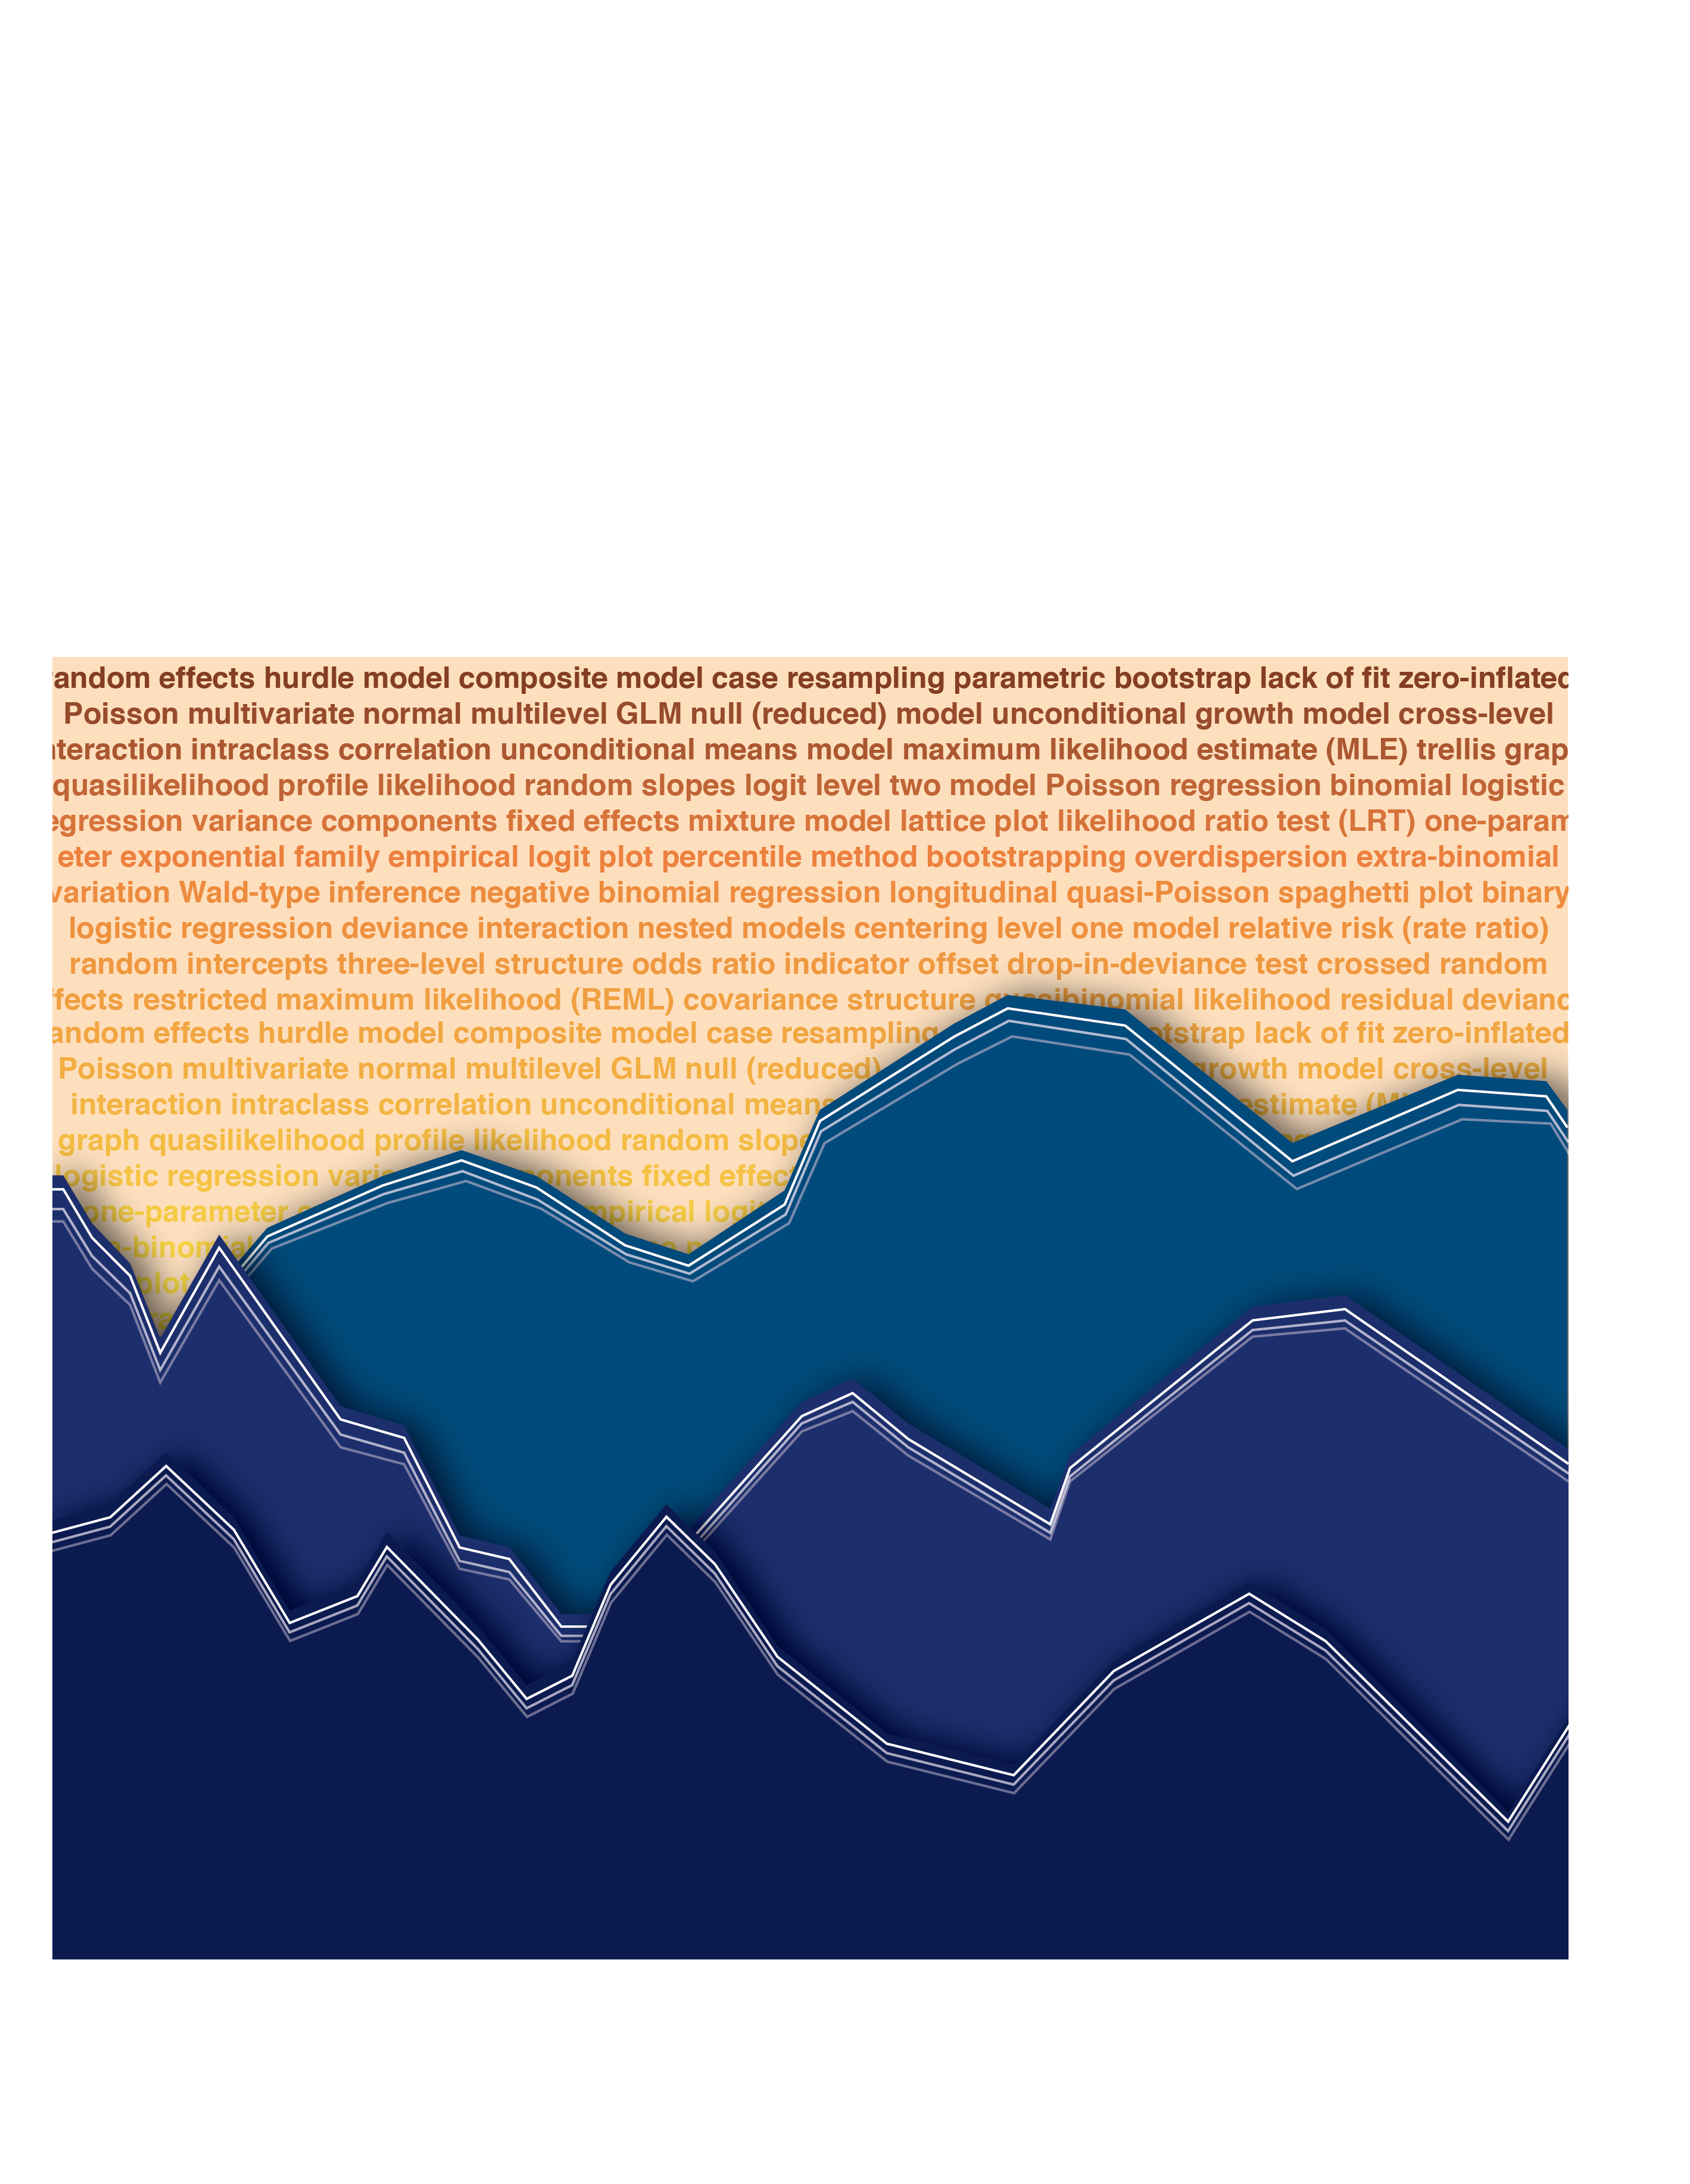
\includegraphics[width=0.75\linewidth]{data/cover}

\textbf{GLMs and Multilevel Models: Broadening Your Statistical Horizons (BYSH) with Applications using R} is intended to be accessible to undergraduate students who have successfully completed a regression course through, for example, a textbook like \emph{Stat2} \citep{Cannon2019}. We started teaching this course at St.~Olaf in 2003 so students would be able to deal with the non-normal, correlated world we live in. It has been offered at St.~Olaf every year since. Even though there is no mathematical prerequisite, we still introduce fairly sophisticated topics such as likelihood theory, zero-inflated Poisson, and parametric bootstrapping in an intuitive and applied manner. We believe strongly in case studies featuring real data and real research questions; thus, most of the data in the textbook and \href{https://github.com/proback/BYSH}{available at our GitHub repo} arises from collaborative research conducted by the authors and their students, or from student projects. Our goal is that, after working through this material, students will not necessarily be expert in these methods and associated theory, but that they will develop an expanded toolkit and a greater appreciation for the wider world of data and statistical modeling.

This work is licensed under a Creative Commons Attribution-NonCommercial-ShareAlike 4.0 International License.

\textbf{Acknowledgements.} We would like to thank students of Stat 316 at St.~Olaf College since 2010 for their patience as this book has taken shape with their feedback. We would especially like to thank these St.~Olaf students for their summer research efforts which significantly improved aspects of this book: Cecilia Noecker, Anna Johanson, Nicole Bettes, Kiegan Rice, Anna Wall, Jack Wolf, Josh Pelayo, Spencer Eanes, and Emily Patterson. Early editions of this book also benefitted greatly from feedback from instructors who used these materials in their classes, including Matt Beckman, Laura Boehm Vock, Beth Chance, Laura Chihara, Mine Dogucu, and Katie Ziegler-Graham. Finally, we have appreciated the support of two NSF grants (\#DMS-1045015 and \#DMS-0354308) and of our colleagues in Mathematics, Statistics, and Computer Science at St.~Olaf.

\hypertarget{ch-lon}{%
\chapter{Two Level Longitudinal Data}\label{ch-lon}}

\hypertarget{learning-objectives}{%
\section{Learning objectives}\label{learning-objectives}}

After finishing this chapter, you should be able to:

\begin{itemize}
\tightlist
\item
  Recognize longitudinal data as a special case of multilevel data, with time at Level One.
\item
  Consider patterns of missingness and implications of that missing data on multilevel analyses.
\item
  Apply exploratory data analysis techniques specific to longitudinal data.
\item
  Build and understand a taxonomy of models for longitudinal data.
\item
  Interpret model parameters in multilevel models with time at Level One.
\item
  Compare models, both nested and not, with appropriate statistical tests and summary statistics.
\item
  Consider different ways of modeling the variance-covariance structure in longitudinal data.
\end{itemize}

\begin{Shaded}
\begin{Highlighting}[]
\CommentTok{# Packages required for Chapter 9}
\KeywordTok{library}\NormalTok{(GGally)}
\KeywordTok{library}\NormalTok{(data.table)}
\KeywordTok{library}\NormalTok{(Hmisc)}
\KeywordTok{library}\NormalTok{(mice)}
\KeywordTok{library}\NormalTok{(lattice)}
\KeywordTok{library}\NormalTok{(nlme)}
\KeywordTok{library}\NormalTok{(reshape2)}
\KeywordTok{library}\NormalTok{(MASS)}
\KeywordTok{library}\NormalTok{(mnormt)}
\KeywordTok{library}\NormalTok{(lme4)}
\KeywordTok{library}\NormalTok{(gridExtra) }
\KeywordTok{library}\NormalTok{(knitr)}
\KeywordTok{library}\NormalTok{(kableExtra)}
\KeywordTok{library}\NormalTok{(tidyverse)}
\end{Highlighting}
\end{Shaded}

\hypertarget{cs:charter}{%
\section{Case study: Charter schools}\label{cs:charter}}

Charter schools were first introduced in the state of Minnesota in 1991 \citep{CharterSchools}. Since then, charter schools have begun appearing all over the United States. While publicly funded, a unique feature of charter schools is their independence from many of the regulations that are present in the public school systems of their respective city or state. Thus, charters will often extend the school days or year and tend to offer non-traditional techniques and styles of instruction and learning.

One example of this unique schedule structure is the KIPP (Knowledge is Power Program) Stand Academy in Minneapolis, MN. KIPP stresses longer days and better partnerships with parents, and they claim that 80\% of their students go to college from a population where 87\% qualify for free and reduced lunch and 95\% are African-American or Latino \citep{KIPP}. However, the larger question is whether or not charter schools are out-performing non-charter public schools in general. Because of the relative youthfulness of charter schools, data has just begun to be collected to evaluate the performance of charter versus non-charter schools and some of the factors that influence a school's performance. Along these lines, we will examine data collected by the Minnesota Department of Education for all Minnesota schools during the years 2008-2010.

Comparisons of student performance in charter schools versus public schools have produced conflicting results, potentially as a result of the strong differences in the structure and population of the student bodies that represent the two types of schools. A study by the Policy and Program Studies Service of five states found that charter schools are less likely to meet state performance standards than conventional public schools \citep{DepartmentOfEducation2004}. However, \citet{Witte2007} performed a statistical analysis comparing Wisconsin charter and non-charter schools and found that average achievement test scores were significantly higher in charter schools compared to non-charter schools, after controlling for demographic variables such as the percentage of white students. In addition, a study of California students who took the Stanford 9 exam from 1998 through 2002 found that charter schools, on average, were performing at the same level as conventional public schools \citep{Buddin2005}. Although school performance is difficult to quantify with a single measure, for illustration purposes in this chapter we will focus on that aspect of school performance measured by the math portion of the Minnesota Comprehensive Assessment (MCA-II) data for 6th grade students enrolled in 618 different Minnesota schools during the years 2008, 2009, and 2010 \citep{MNDepartmentOfEducation}. Similar comparisons could obviously be conducted for other grade levels or modes of assessment.

As described in \citet{Green2003}, it is very challenging to compare charter and public non-charter schools, as charter schools are often designed to target or attract specific populations of students. Without accounting for differences in student populations, comparisons lose meaning. With the assistance of multiple school-specific predictors, we will attempt to model sixth grade math MCA-II scores of Minnesota schools, focusing on the differences between charter and public non-charter school performances. In the process, we hope to answer the following research questions:

\begin{itemize}
\tightlist
\item
  Which factors most influence a school's performance in MCA testing?
\item
  How do the average math MCA-II scores for 6th graders enrolled in charter schools differ from scores for students who attend non-charter public schools? Do these differences persist after accounting for differences in student populations?
\item
  Are there differences in yearly improvement between charter and non-charter public schools?
\end{itemize}

\hypertarget{exploratoryanalysis}{%
\section{Initial Exploratory Analyses}\label{exploratoryanalysis}}

\hypertarget{data}{%
\subsection{Data organization}\label{data}}

Key variables in \texttt{chart\_wide\_condense.csv} which we will examine to address the research questions above are:

\begin{itemize}
\tightlist
\item
  \texttt{schoolid} = includes district type, district number, and school number
\item
  \texttt{schoolName} = name of school
\item
  \texttt{urban} = is the school in an urban (1) or rural (0) location?
\item
  \texttt{charter} = is the school a charter school (1) or a non-charter public school (0)?
\item
  \texttt{schPctnonw} = proportion of non-white students in a school (based on 2010 figures)
\item
  \texttt{schPctsped} = proportion of special education students in a school (based on 2010 figures)
\item
  \texttt{schPctfree} = proportion of students who receive free or reduced lunches in a school (based on 2010 figures). This serves as a measure of poverty among school families.
\item
  \texttt{MathAvgScore.0} = average MCA-II math score for all sixth grade students in a school in 2008
\item
  \texttt{MathAvgScore.1} = average MCA-II math score for all sixth grade students in a school in 2009
\item
  \texttt{MathAvgScore.2} = average MCA-II math score for all sixth grade students in a school in 2010
\end{itemize}

This data is stored in WIDE format, with one row per school, as illustrated in Table \ref{tab:table1chp9}.

\begin{table}

\caption{\label{tab:table1ch9}The first six observations in the wide data set for the Charter Schools case study.}
\centering
\resizebox{\linewidth}{!}{
\begin{tabular}[t]{llrrrrrrrr}
\toprule
schoolid & schoolName & urban & charter & schPctnonw & schPctsped & schPctfree & MathAvgScore.0 & MathAvgScore.1 & MathAvgScore.2\\
\midrule
Dtype 1 Dnum 1 Snum 2 & RIPPLESIDE ELEMENTARY & 0 & 0 & 0.0000 & 0.1176 & 0.3627 & 652.8 & 656.6 & 652.6\\
Dtype 1 Dnum 100 Snum 1 & WRENSHALL ELEMENTARY & 0 & 0 & 0.0303 & 0.1515 & 0.4242 & 646.9 & 645.3 & 651.9\\
Dtype 1 Dnum 108 Snum 30 & CENTRAL MIDDLE & 0 & 0 & 0.0769 & 0.1231 & 0.2615 & 654.7 & 658.5 & 659.7\\
Dtype 1 Dnum 11 Snum 121 & SANDBURG MIDDLE & 1 & 0 & 0.0977 & 0.0827 & 0.2481 & 656.4 & 656.8 & 659.9\\
Dtype 1 Dnum 11 Snum 193 & OAK VIEW MIDDLE & 1 & 0 & 0.0538 & 0.0954 & 0.1418 & 657.7 & 658.2 & 659.8\\
\addlinespace
Dtype 1 Dnum 11 Snum 195 & ROOSEVELT MIDDLE & 1 & 0 & 0.1234 & 0.0886 & 0.2405 & 655.9 & 659.1 & 660.3\\
\bottomrule
\end{tabular}}
\end{table}

For most statistical analyses, it will be advantageous to convert WIDE format to LONG format, with one row per year per school. To make this conversion, we will have to create a time variable, which under the LONG format is very flexible---each school can have a different number of and differently-spaced time points, and they can even have predictors which vary over time. Details for making this conversion in R can be found in Section \ref{notesr9}, and the form of the LONG data in this study is exhibited in the next section.

\hypertarget{missing}{%
\subsection{Missing data}\label{missing}}

In this case, before we convert our data to LONG form, we should first address problems with missing data. Missing data is a common phenomenon in longitudinal studies. For instance, it could arise if a new school was started during the observation period, a school was shut down during the observation period, or no results were reported in a given year. Dealing with missing data in a statistical analysis is not trivial, but fortunately many multilevel packages (including the lme4 package in R) are adept at handling missing data.

First, we must understand the extent and nature of missing data in our study. Table \ref{tab:table2chp9}, where 1 indicates presence of a variable and 0 indicates a missing value for a particular variable, is a helpful starting point. Among our 618 schools, 540 had complete data (all covariates and math scores for all three years), 25 were missing a math score for 2008, 35 were missing math scores in both 2008 and 2009, etc.

\label{tab:table2chp9} A frequency table of missing data patterns. The number of schools with a particular missing data pattern are listed in the left column; the remaining columns of 0's and 1's describe the missing data pattern, with 0 indicating a missing value. Some covariates that are present for every school are not listed. The bottom row gives the number of schools with missing values for specific variables; the last entry indicates that 121 total observations were missing.

\begin{table}

\caption{\label{tab:table2chp9}A frequency table of missing data patterns. The number of schools with a particular missing data pattern are listed in the left column; the remaining columns of 0's and 1's describe the missing data pattern, with 0 indicating a missing value.  Some covariates that are present for every school are not listed.  The bottom row gives the number of schools with missing values for specific variables; the last entry indicates that 121 total observations were missing.}
\centering
\resizebox{\linewidth}{!}{
\begin{tabular}[t]{lrrrrr}
\toprule
  & charter & MathAvgScore.2 & MathAvgScore.1 & MathAvgScore.0 & \\
\midrule
540 & 1 & 1 & 1 & 1 & 0\\
25 & 1 & 1 & 1 & 0 & 1\\
4 & 1 & 1 & 0 & 1 & 1\\
35 & 1 & 1 & 0 & 0 & 2\\
6 & 1 & 0 & 1 & 1 & 1\\
\addlinespace
1 & 1 & 0 & 1 & 0 & 2\\
7 & 1 & 0 & 0 & 1 & 2\\
 & 0 & 14 & 46 & 61 & 121\\
\bottomrule
\end{tabular}}
\end{table}

Statisticians have devised different strategies for handling missing data; a few common approaches are described briefly here:

\begin{itemize}
\tightlist
\item
  Include only schools with complete data. This is the cleanest approach analytically; however, ignoring data from 12.6\% of the study's schools (since 78 of the 618 schools had incomplete data) means that a large amount of potentially useful data is being thrown away. In addition, this approach creates potential issues with informative missingness. Informative missingness occurs when a school's lack of scores is not a random phenomenon but provides information about the effectiveness of the school type (e.g., a school closes because of low test scores).
\item
  Last observation carried forward. Each school's last math score is analyzed as a univariate response, whether the last measurement was taken in 2008, 2009, or 2010. With this approach, data from all schools can be used, and analyses can be conducted with traditional methods assuming independent responses. This approach is sometimes used in clinical trials because it tends to be conservative, setting a higher bar for showing that a new therapy is significantly better than a traditional therapy. Of course, we must assume that a school's 2008 score is representative of their 2010 score. In addition, information about trajectories over time is thrown away.
\item
  Imputation of missing observations. Many methods have been developed for sensibly ``filling in'' missing observations, using imputation models which base imputed data on subjects with similar covariate profiles and on typical observed time trends. Once an imputed data set is created (or several imputed data sets), analyses can proceed with complete data methods that are easier to apply. Risks with the imputation approach include misrepresenting missing observations and overstating precision in final results.
\item
  Apply multilevel methods, which use available data to estimate patterns over time by school and then combine those school estimates in a way that recognizes that time trends for schools with complete data are more precise than time trends for schools with fewer measurements. \citet{Laird1988} demonstrates that multilevel models are valid under the fairly unrestrictive condition that the probability of missingness cannot depend on any unobserved predictors or the response. This is the approach we will follow in the remainder of the text.
\end{itemize}

Now, we are ready to create our LONG data set. Fortunately, many packages (including R) have built-in functions for easing this conversion, and the functions are improving constantly. The resulting LONG data set is shown in Table \ref{tab:table3chp9}, where \texttt{year08} measures the number of years since 2008:



\begin{table}

\caption{\label{tab:table3chp9}The first six observations in the long data set for the Charter Schools case study; these lines correspond to the first two observations from the wide data set illustrated in Table \ref{tab:table1chp9}.}
\centering
\resizebox{\linewidth}{!}{
\begin{tabular}[t]{lrrrrr}
\toprule
schoolName & charter & schPctsped & schPctfree & year08 & MathAvgScore\\
\midrule
RIPPLESIDE ELEMENTARY & 0 & 0.1176 & 0.3627 & 0 & 652.8\\
RIPPLESIDE ELEMENTARY & 0 & 0.1176 & 0.3627 & 1 & 656.6\\
RIPPLESIDE ELEMENTARY & 0 & 0.1176 & 0.3627 & 2 & 652.6\\
WRENSHALL ELEMENTARY & 0 & 0.1515 & 0.4242 & 0 & 646.9\\
WRENSHALL ELEMENTARY & 0 & 0.1515 & 0.4242 & 1 & 645.3\\
\addlinespace
WRENSHALL ELEMENTARY & 0 & 0.1515 & 0.4242 & 2 & 651.9\\
\bottomrule
\end{tabular}}
\end{table}

\hypertarget{generalanalyses}{%
\subsection{Exploratory analyses for general multilevel models}\label{generalanalyses}}

Notice the \textbf{longitudinal} structure of our data---we have up to three measurements of test scores at different time points for each of our 618 schools. With this structure, we can address questions at two levels:

\begin{itemize}
\tightlist
\item
  Within school---changes over time
\item
  Between schools---effects of school-specific covariates (charter or non-charter, urban or rural, percent free and reduced lunch, percent special education, and percent non-white) on 2008 math scores and rate of change between 2008 and 2010.
\end{itemize}

As with any statistical analysis, it is vitally important to begin with graphical and numerical summaries of important variables and relationships between variables. We'll begin with initial exploratory analyses that we introduced in the previous chapter, noting that we have no Level One covariates other than time at this point (potential covariates at this level may have included measures of the number of students tested or funds available per student). We will, however, consider the Level Two variables of charter or non-charter, urban or rural, percent free and reduced lunch, percent special education, and percent non-white. Although covariates such as percent free and reduced lunch may vary slightly from year to year within a school, the larger and more important differences tend to occur between schools, so we used percent free and reduced lunch for a school in 2010 as a Level Two variable.

As in Chapter \ref{ch-multilevelintro}, we can conduct initial investigations of relationships between Level Two covariates and test scores in two ways. First, we can use all 1733 observations to investigate relationships of Level Two covariates with test scores. Although these plots will contain dependent points, since each school is represented by up to three years of test score data, general patterns exhibited in these plots tend to be real. Second, we can calculate mean scores across all years for each of the 618 schools. While we lose some information with this approach, we can more easily consider each plotted point to be independent. Typically, both types of exploratory plots illustrate similar relationships, and in this case, both approaches are so similar that we will only show plots using the second approach, with one observation per school.

Figure \ref{fig:lon-hist1} shows the distribution of MCA math test scores as somewhat left skewed. MCA test scores for sixth graders are scaled to fall between 600 and 700, where scores above 650 for individual students indicate ``meeting standards''. Thus, schools with averages below 650 will often have increased incentive to improve their scores the following year. When we refer to the ``math score'' for a particular school in a particular year, we will assume that score represents the average for all sixth graders at that school. In Figure \ref{fig:lon-box1}, we see that test scores are generally higher for both schools in rural areas and for public non-charter schools. Note that in this data set there are 237 schools in rural areas and 381 schools in urban areas, as well as 545 public non-charter schools and 73 charter schools. In addition, we can see in Figure \ref{fig:lon-scat1} that schools tend to have lower math scores if they have higher percentages of students with free and reduced lunch, with special education needs, or who are non-white.

\begin{figure}

{\centering 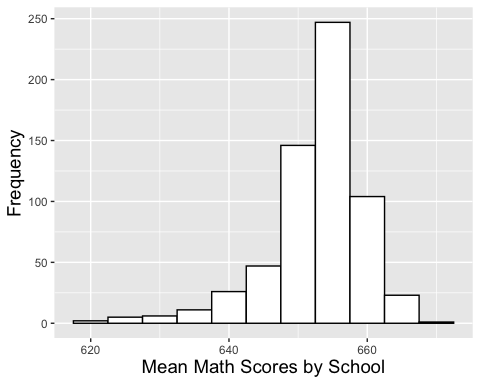
\includegraphics[width=0.6\linewidth]{bookdown-bysh_files/figure-latex/lon-hist1-1} 

}

\caption{Histogram of mean sixth grade MCA math test scores over the years 2008-2010 for 618 Minnesota schools.}\label{fig:lon-hist1}
\end{figure}

\begin{figure}

{\centering 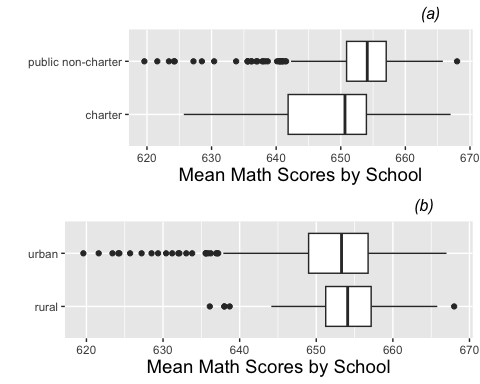
\includegraphics[width=0.6\linewidth]{bookdown-bysh_files/figure-latex/lon-box1-1} 

}

\caption{Boxplots of categorical Level Two covariates vs. average MCA math scores.  Plot (a) shows charter vs. public non-charter schools, while plot (b) shows urban vs. rural schools.}\label{fig:lon-box1}
\end{figure}

\begin{verbatim}
## `geom_smooth()` using formula 'y ~ x'
## `geom_smooth()` using formula 'y ~ x'
## `geom_smooth()` using formula 'y ~ x'
\end{verbatim}

\begin{figure}

{\centering 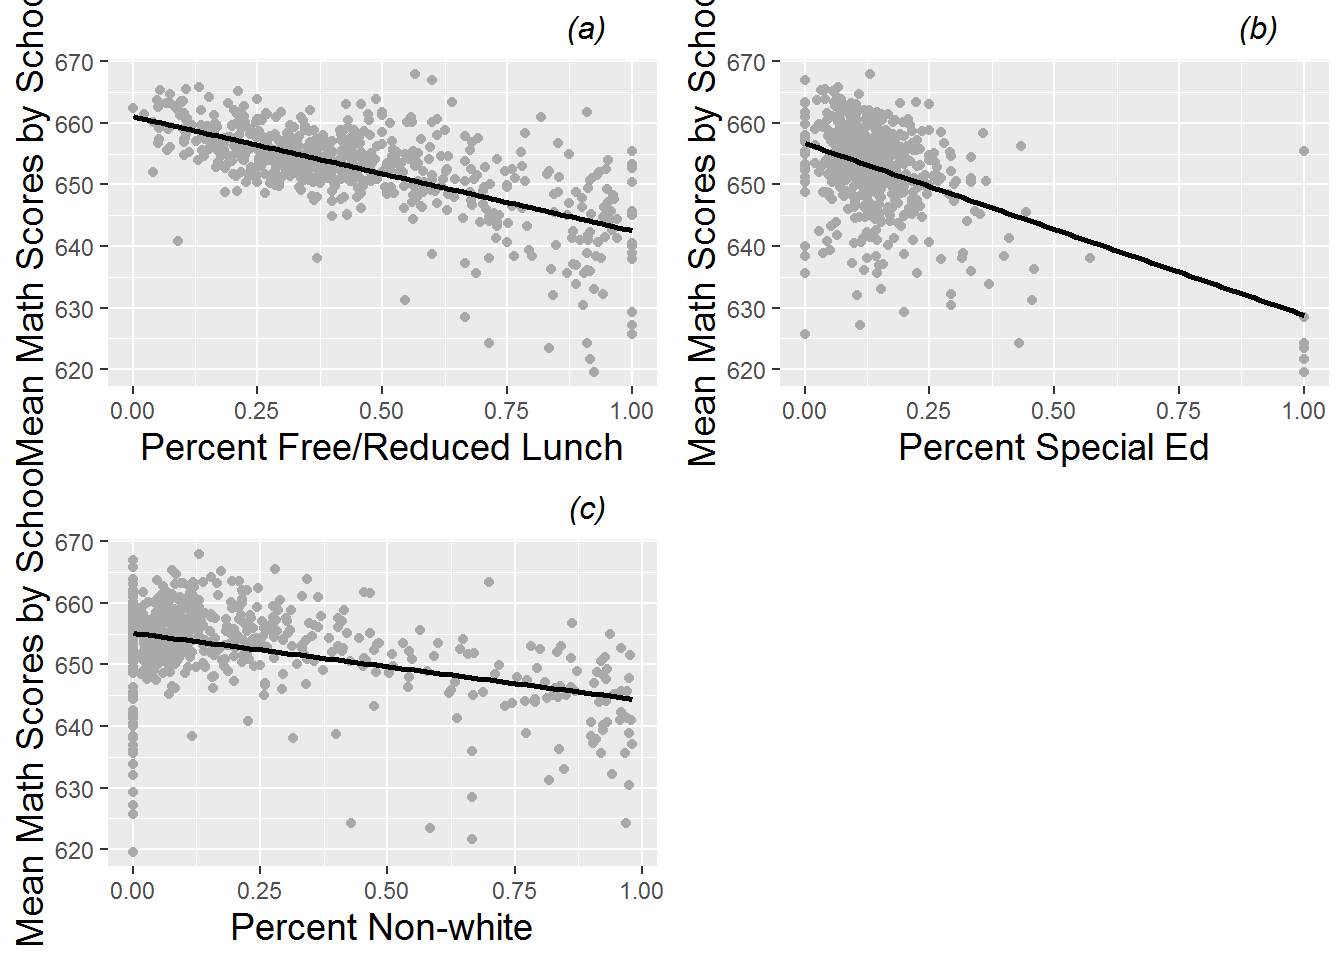
\includegraphics[width=0.6\linewidth]{bookdown-bysh_files/figure-latex/lon-scat1-1} 

}

\caption{ Scatterplots of average MCA math scores by (a) percent free and reduced lunch, (b) percent special education, and (c) percent non-white in a school.}\label{fig:lon-scat1}
\end{figure}

\hypertarget{longitudinalanalyses}{%
\subsection{Exploratory analyses for longitudinal data}\label{longitudinalanalyses}}

In addition to the initial exploratory analyses above, longitudinal data---multilevel data with time at Level One---calls for further plots and summaries that describe time trends within and across individuals. For example, we can examine trends over time within individual schools. Figure \ref{fig:lon-lat1} provides a \textbf{lattice plot} illustrating trends over time for the first 24 schools in the data set. We note differences among schools in starting point (test scores in 2008), slope (change in test scores over the three year period), and form of the relationship. These differences among schools are nicely illustrated in so-called \textbf{spaghetti plots} such as Figure \ref{fig:lon-spag1}, which overlays the individual schools' time trends (for the math test scores) from Figure \ref{fig:lon-lat1} on a single set of axes. In order to illustrate the overall time trend without making global assumptions about the form of the relationship, we overlaid in bold a nonparametric fitted curve through a \textbf{loess smoother}. LOESS comes from ``locally weighted scatterplot smoother'', in which a low-degree polynomial is fit to each data point using weighted regression techniques, where nearby points receive greater weight. LOESS is a computationally intensive method which performs especially well with larger sets of data, although ideally there would be a greater diversity of x-values than the three time points we have. In this case, the loess smoother follows very closely to a linear trend, indicating that assuming a linear increase in test scores over the three year period is probably a reasonable simplifying assumption. To further examine the hypothesis that linearity would provide a reasonable approximation to the form of the individual time trends in most cases, Figure \ref{fig:lon-lat2} shows a lattice plot containing linear fits through ordinary least squares rather than connected time points as in Figure \ref{fig:lon-lat1}.

\begin{figure}

{\centering 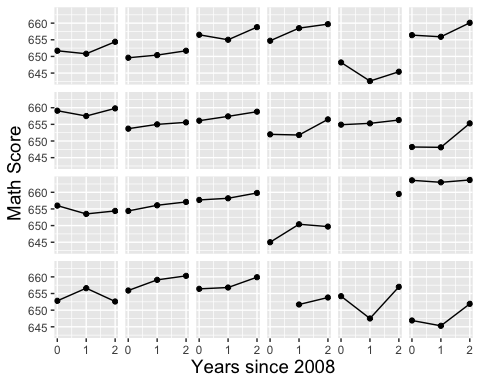
\includegraphics[width=0.6\linewidth]{bookdown-bysh_files/figure-latex/lon-lat1-1} 

}

\caption{Lattice plot by school of math scores over time for the first 24 schools in the data set.}\label{fig:lon-lat1}
\end{figure}

\begin{figure}

{\centering 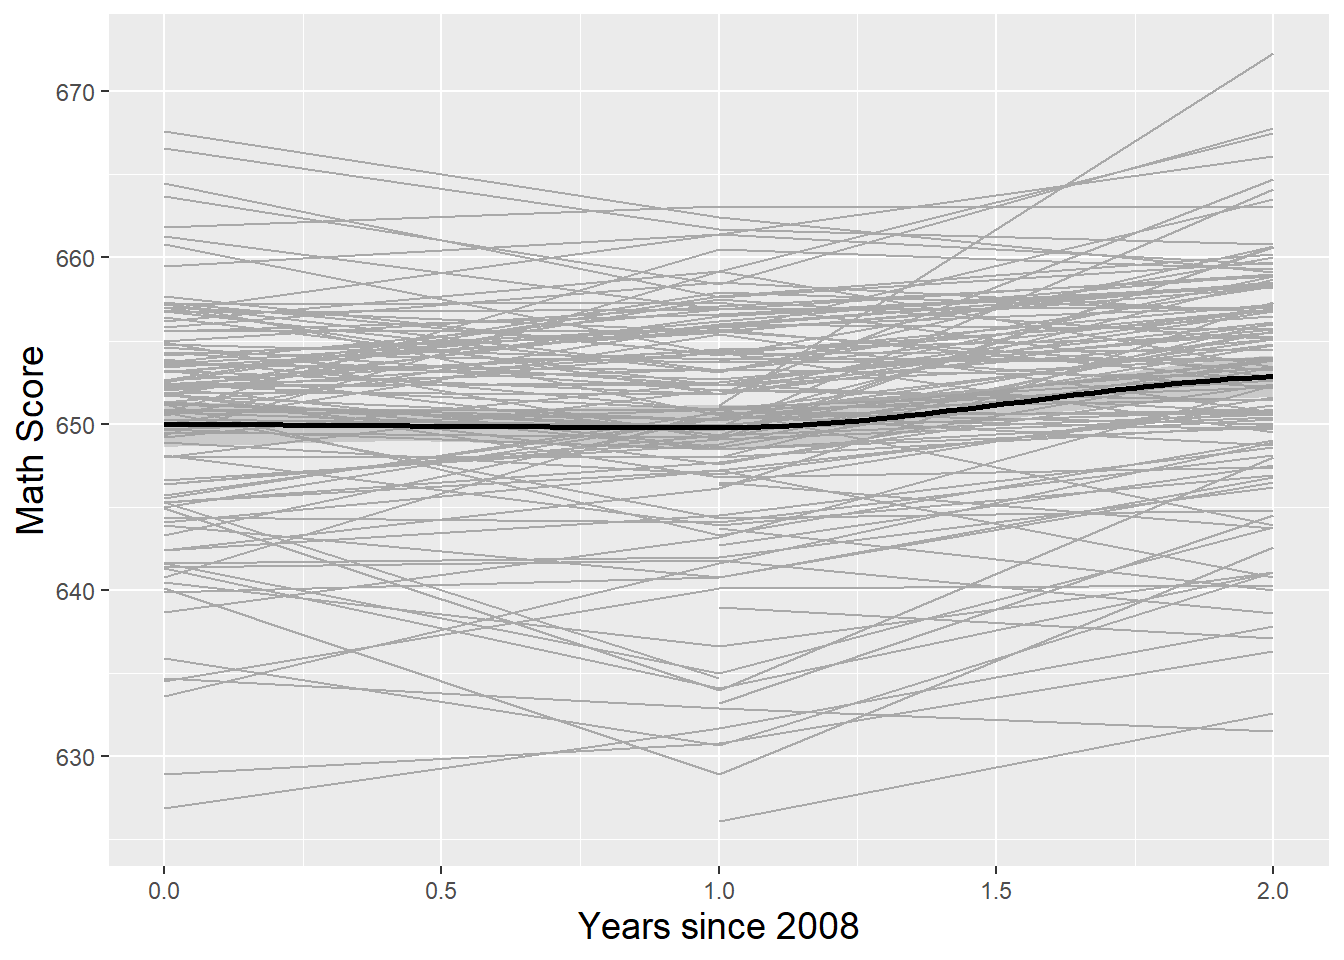
\includegraphics[width=0.6\linewidth]{bookdown-bysh_files/figure-latex/lon-spag1-1} 

}

\caption{ Spaghetti plot of math scores over time by school, for all the charter schools and a random sample of public non-charter schools, with overall fit using loess (bold).}\label{fig:lon-spag1}
\end{figure}

\begin{verbatim}
## `geom_smooth()` using formula 'y ~ x'
\end{verbatim}

\begin{figure}

{\centering 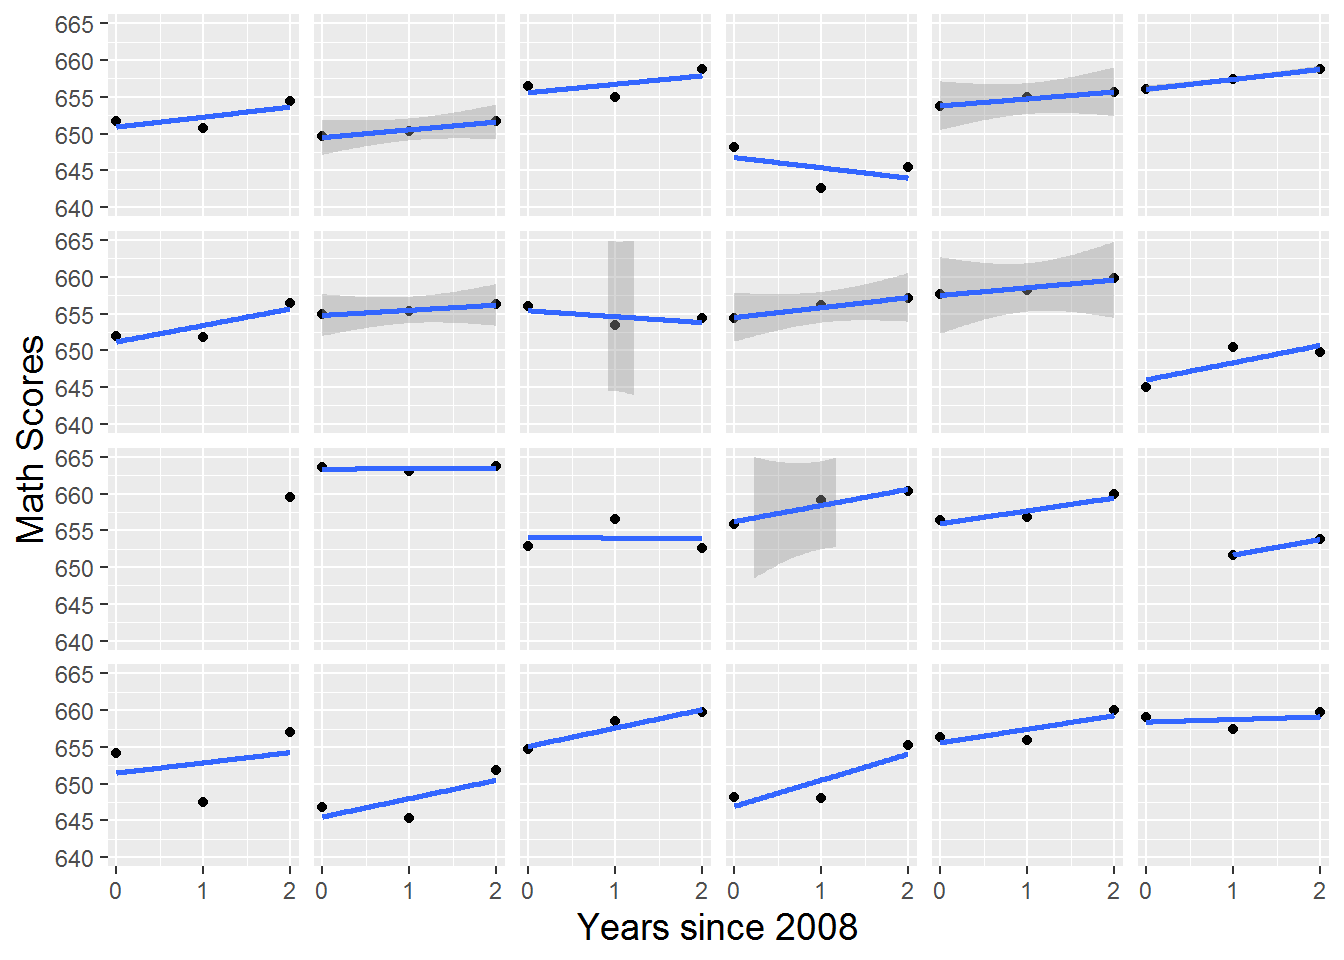
\includegraphics[width=0.6\linewidth]{bookdown-bysh_files/figure-latex/lon-lat2-1} 

}

\caption{ Lattice plot by school of math scores over time with linear fit for the first 24 schools in the data set.}\label{fig:lon-lat2}
\end{figure}

\begin{figure}

{\centering 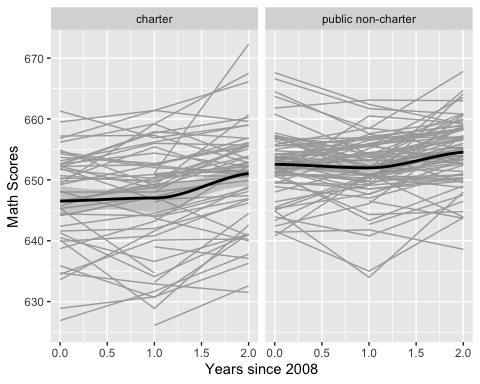
\includegraphics[width=0.6\linewidth]{bookdown-bysh_files/figure-latex/lon-spag3-1} 

}

\caption{Spaghetti plots showing time trends for each school by school type, for a random sample of charter schools (left) and public non-charter schools (right), with overall fits using loess (bold).}\label{fig:lon-spag3}
\end{figure}

\begin{verbatim}
## `geom_smooth()` using formula 'y ~ x'
\end{verbatim}

\begin{figure}

{\centering 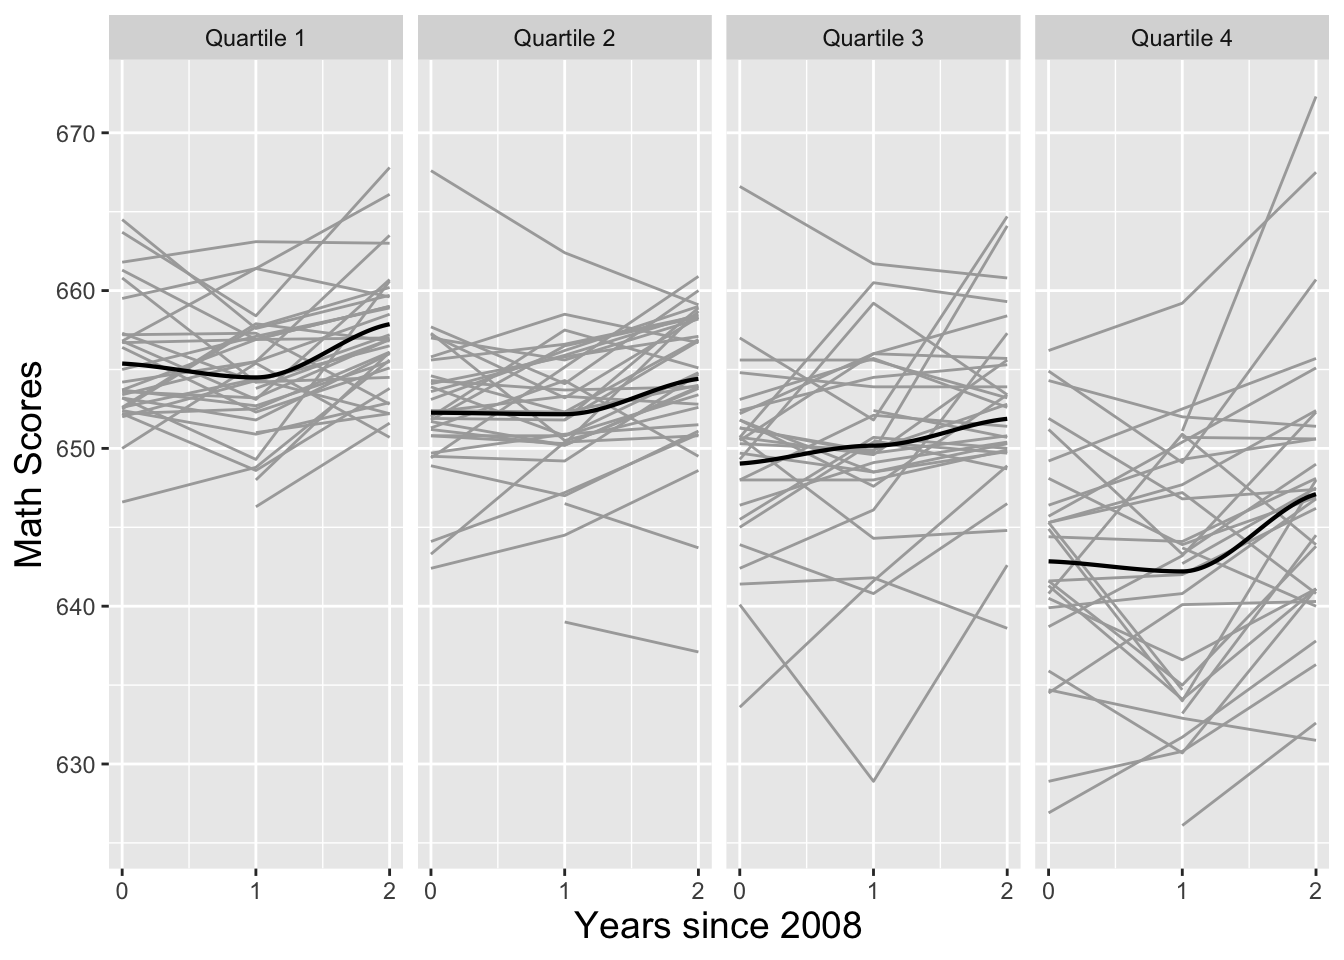
\includegraphics[width=0.6\linewidth]{bookdown-bysh_files/figure-latex/lon-spagmat1-1} 

}

\caption{Spaghetti plots showing time trends for each school by quartiles of percent free and reduced lunch, with loess fits.}\label{fig:lon-spagmat1}
\end{figure}

Just as we explored the relationship between our response (average math scores) and important covariates in Section \ref{generalanalyses}, we can now examine the relationships between time trends by school and important covariates. For instance, Figure \ref{fig:lon-spag3} shows that charter schools had math scores that were lower on average than public non-charter schools and more variable. This type of plot is sometimes called a \textbf{trellis graph}, since it displays a grid of smaller charts with consistent scales, where each smaller chart represents a condition---an item in a category. Trends over time by school type are denoted by bold loess curves. Public non-charter schools have higher scores across all years; both school types show little growth between 2008 and 2009, but greater growth between 2009 and 2010, especially charter schools. Exploratory analyses like this can be repeated for other covariates, such as percent free and reduced lunch in Figure \ref{fig:lon-spagmat1}. The trellis plot automatically divides schools into four groups based on quartiles of their percent free and reduced lunch, and we see that schools with lower percentages of free and reduced lunch students tend to have higher math scores and less variability. Across all levels of free and reduced lunch, we see greater gains between 2009 and 2010 than between 2008 and 2009.

\hypertarget{twostage9}{%
\section{Preliminary two-stage modeling}\label{twostage9}}

\hypertarget{lineartwostage}{%
\subsection{Linear trends within schools}\label{lineartwostage}}

Even though we know that every school's math test scores were not strictly linearly increasing or decreasing over the observation period, a linear model for individual time trends is often a simple but reasonable way to model data. One advantage of using a linear model within school is that each school's data points can be summarized with two summary statistics---an intercept and a slope (obviously, this is an even bigger advantage when there are more observations over time per school). For instance, we see in Figure \ref{fig:lon-lat2} that sixth graders from the school depicted in the top right slot slowly increased math scores over the three year observation period, while students from the school depicted in the fourth column of the top row generally experienced decreasing math scores over the same period. As a whole, the linear model fits individual trends pretty well, and many schools appear to have slowly increasing math scores over time, as researchers in this study may have hypothesized.

Another advantage of assuming a linear trend at Level One (within schools) is that we can examine summary statistics across schools. Both the intercept and slope are meaningful for each school: the \emph{intercept} conveys the school's math score in 2008, while the \emph{slope} conveys the school's average yearly increase or decrease in math scores over the three year period. Figure \ref{fig:lon-cis1} shows that point estimates and uncertainty surrounding individual estimates of intercepts and slopes vary considerably. In addition, we can generate summary statistics and histograms for the 618 intercepts and slopes produced by fitting linear regression models at Level One, in addition to R-square values which describe the strength of fit of the linear model for each school (Figure \ref{fig:lon-histmat1}). For our 618 schools, the mean math score for 2008 was 651.4 (SD=7.28), and the mean yearly rate of change in math scores over the three year period was 1.30 (SD=2.51). We can further examine the relationship between schools' intercepts and slopes. Figure \ref{fig:lon-scat5} shows a general decreasing trend, suggesting that schools with lower 2008 test scores tend to have greater growth in scores between 2008 and 2010 (potentially because those schools have more room for improvement); this trend is supported with a correlation coefficient of -0.32 between fitted intercepts and slopes. Note that, with only 3 or fewer observations for each school, extreme or intractable values for the slope and R-square are possible. For example, slopes cannot be estimated for those schools with just a single test score, R-square values cannot be calculated for those schools with no variability in test scores between 2008 and 2010, and R-square values must be 1 for those schools with only two test scores.



\begin{figure}

{\centering 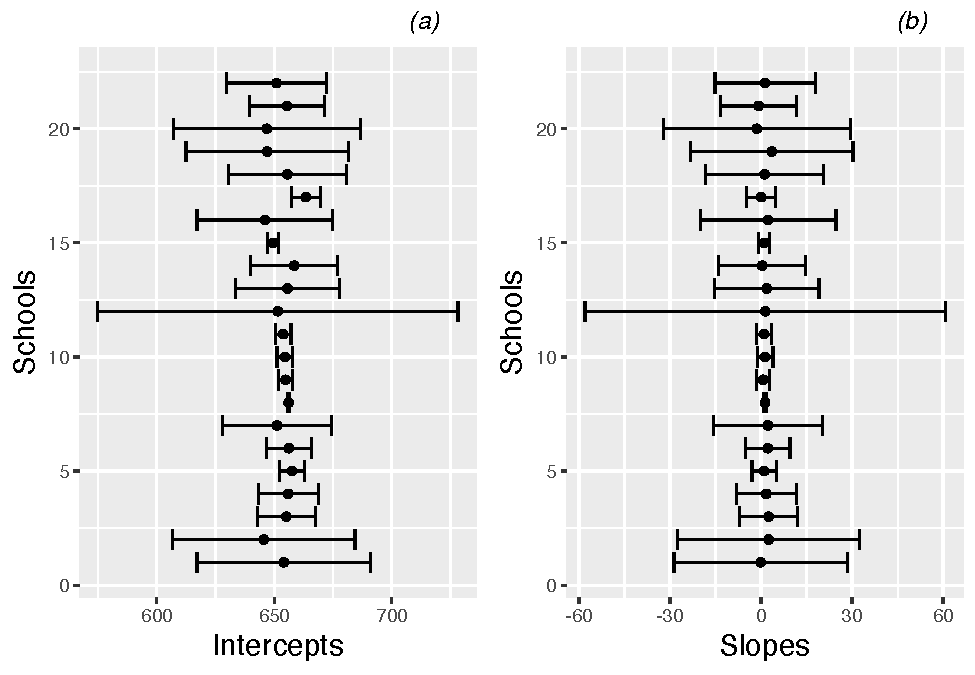
\includegraphics[width=0.6\linewidth]{bookdown-bysh_files/figure-latex/lon-cis1-1} 

}

\caption{Point estimates and 95\% confidence intervals for (a) intercepts and (b) slopes by school, for the first 24 schools in the data set.}\label{fig:lon-cis1}
\end{figure}

\begin{figure}

{\centering 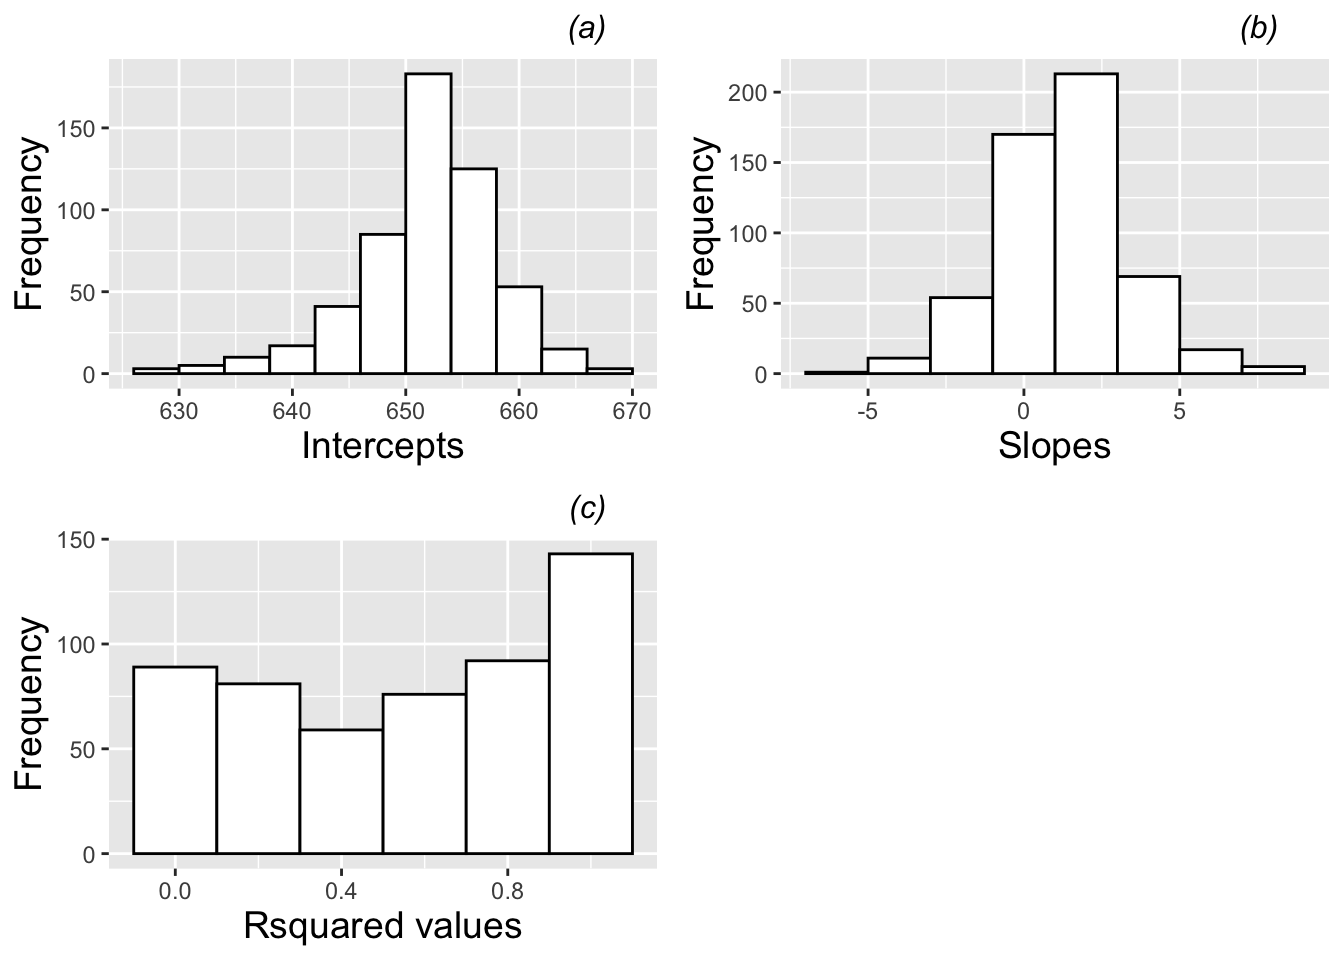
\includegraphics[width=0.6\linewidth]{bookdown-bysh_files/figure-latex/lon-histmat1-1} 

}

\caption{ Histograms for (a) intercepts, (b) slopes, and (c) R-square values from fitted regression lines by school.}\label{fig:lon-histmat1}
\end{figure}

\begin{verbatim}
## `geom_smooth()` using formula 'y ~ x'
\end{verbatim}

\begin{figure}

{\centering 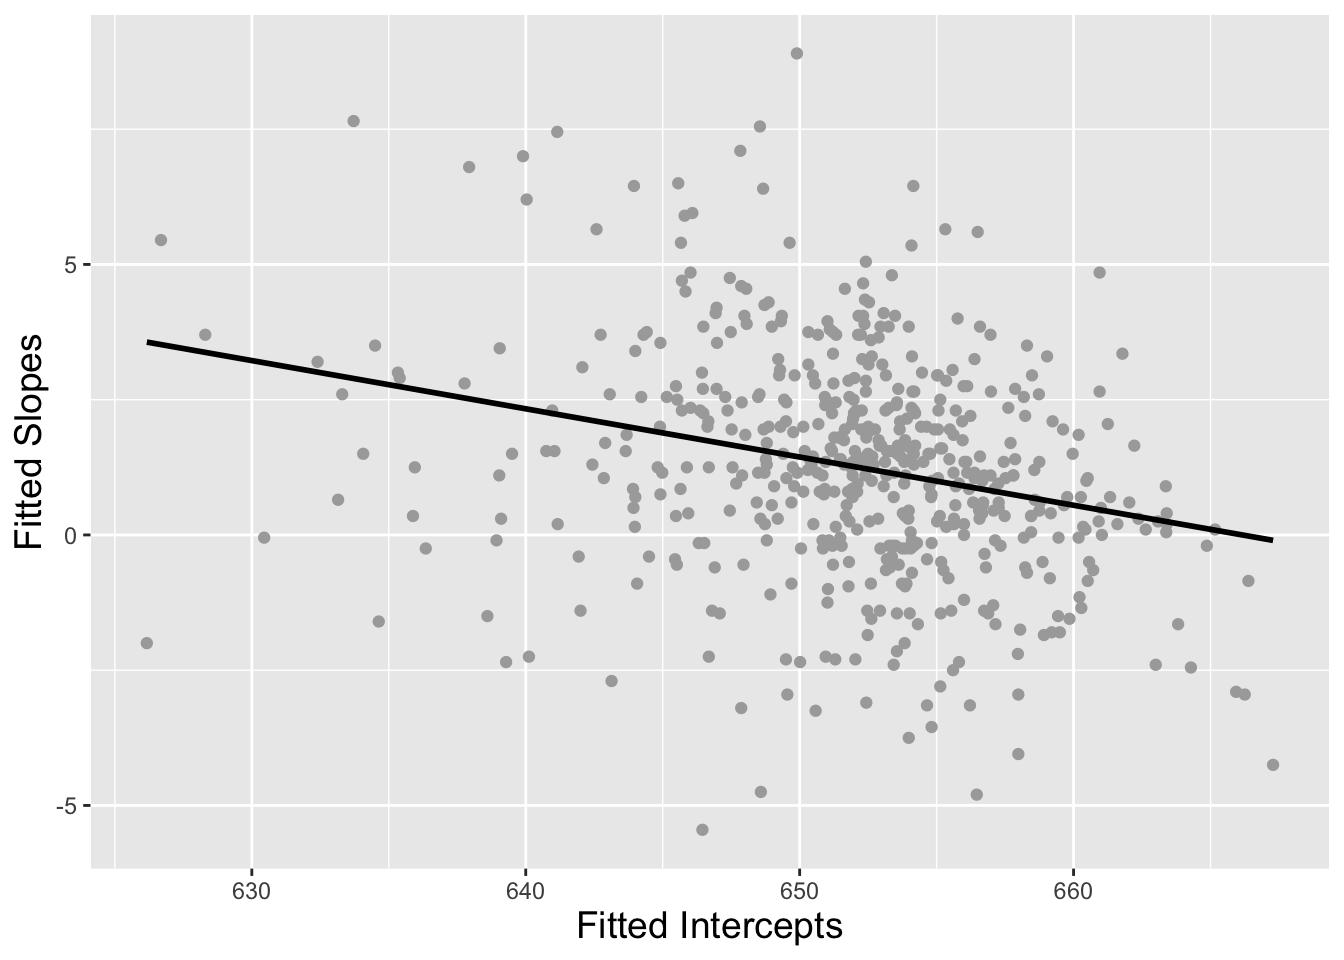
\includegraphics[width=0.6\linewidth]{bookdown-bysh_files/figure-latex/lon-scat5-1} 

}

\caption{Scatterplot showing the relationship between intercepts and slopes from fitted regression lines by school.}\label{fig:lon-scat5}
\end{figure}

\hypertarget{lineartwostageL2effects}{%
\subsection{Effects of level two covariates on linear time trends}\label{lineartwostageL2effects}}

Summarizing trends over time within schools is typically only a start, however. Most of the primary research questions from this study involve comparisons among schools, such as: (a) are there significant differences between charter schools and public non-charter schools, and (b) do any differences between charter schools and public schools change with percent free and reduced lunch, percent special education, or location? These are Level Two questions, and we can begin to explore these questions by graphically examining the effects of school-level variables on schools' linear time trends. By school-level variables, we are referring to those covariates that differ by school but are not dependent on time. For example school type (charter or public non-charter), urban or rural location, percent non-white, percent special education, and percent free and reduced lunch are all variables which differ by school but which don't change over time, at least as they were assessed in this study. Variables which would be time-dependent include quantities such as per pupil funding and reading scores.

Figure \ref{fig:lon-box2} shows differences in the average time trends by school type, using estimated intercepts and slopes to support observations from the spaghetti plots in Figure \ref{fig:lon-spag3}. Based on intercepts, charter schools have lower math scores, on average, in 2008 than public non-charter schools. Based on slopes, however, charter schools tend to improve their math scores at a slightly faster rate than public schools, especially at the seventy-fifth percentile and above. By the end of the three year observation period we would nevertheless expect charter schools to have lower average math scores than public schools. For another exploratory perspective on school type comparisons, we can examine differences between school types with respect to math scores in 2008 and math scores in 2010. As expected, boxplots by school type (Figure \ref{fig:lon-box3}) show clearly lower math scores for charter schools in 2008, but differences are slightly less dramatic in 2010.

\begin{figure}

{\centering 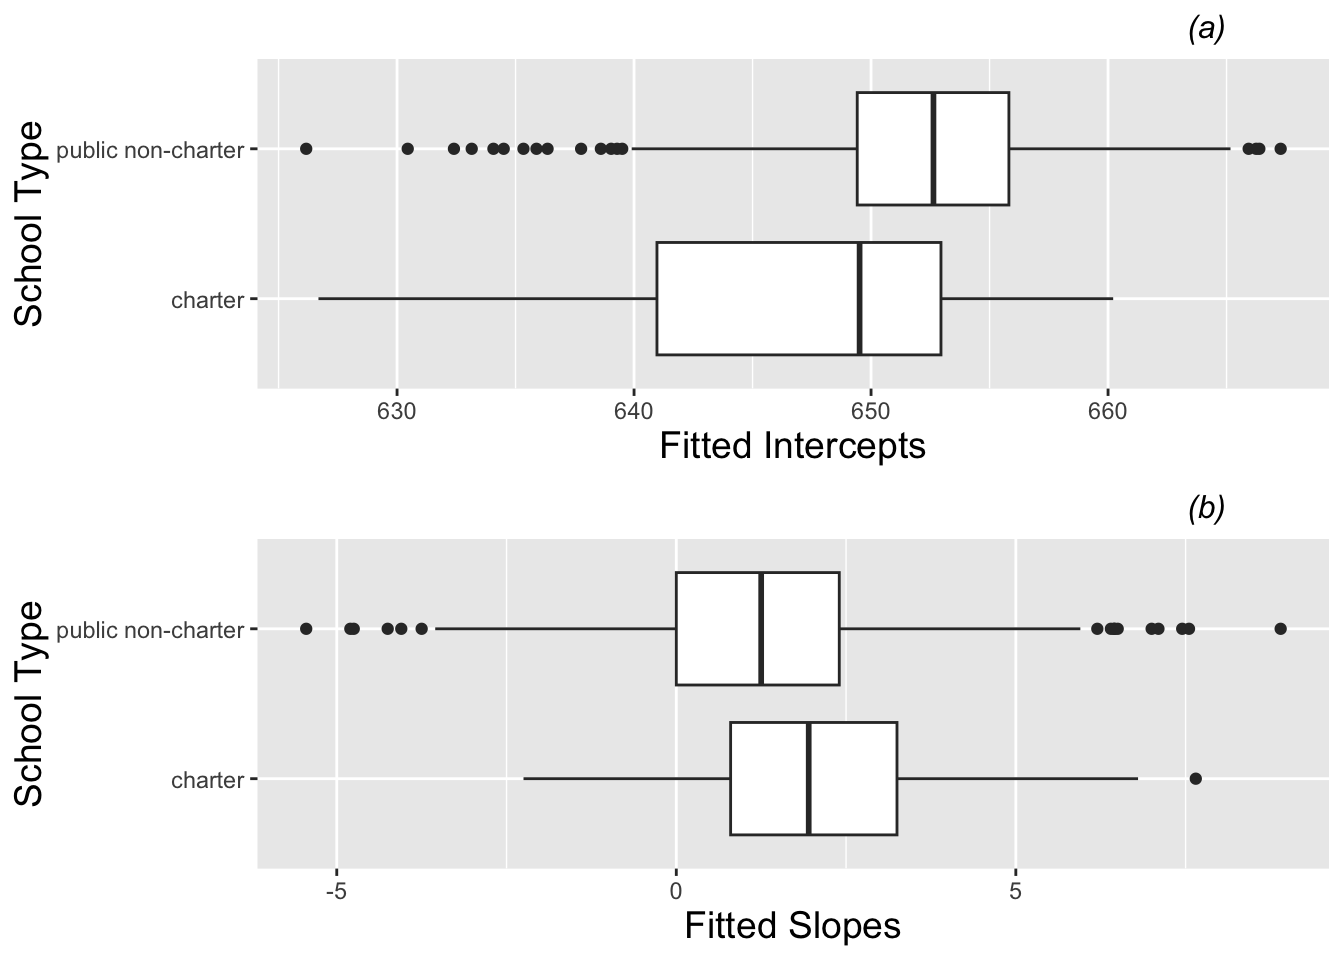
\includegraphics[width=0.6\linewidth]{bookdown-bysh_files/figure-latex/lon-box2-1} 

}

\caption{Boxplots of (a) intercepts and (b) slopes by school type (charter vs. public non-charter).}\label{fig:lon-box2}
\end{figure}

\begin{figure}

{\centering 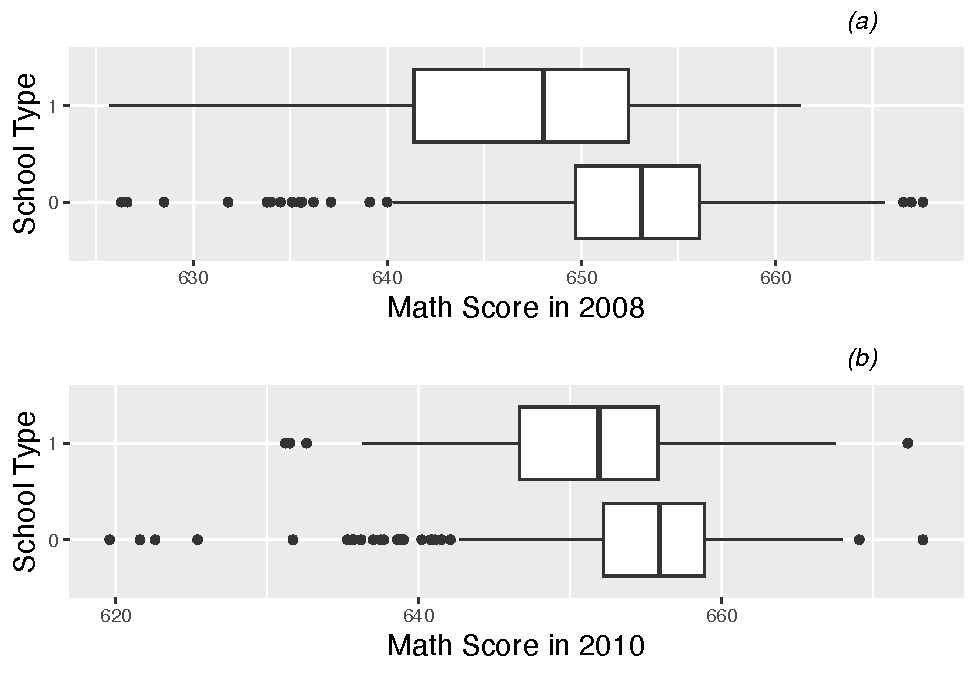
\includegraphics[width=0.6\linewidth]{bookdown-bysh_files/figure-latex/lon-box3-1} 

}

\caption{Boxplots of (a) 2008 and (b) 2010 math scores by school type (charter vs. public non-charter).}\label{fig:lon-box3}
\end{figure}

Any initial exploratory analyses should also investigate effects of potential confounding variables such as school demographics and location. If we discover, for instance, that those schools with higher levels of poverty (measured by the percentage of students receiving free and reduced lunch) display lower test scores in 2008 but greater improvements between 2008 and 2010, then we might be able to use percentage of free and reduced lunch in statistical modeling of intercepts and slopes, leading to more precise estimates of the charter school effects on these two outcomes. In addition, we should also look for any interaction with school type---any evidence that the difference between charter and non-charter schools changes based on the level of a confounding variable. For example, do charter schools perform better relative to non-charter schools when there is a large percentage of non-white students at a school?

With a confounding variable such as percentage of free and reduced lunch, we will treat this variable as continuous to produce the most powerful exploratory analyses. We can begin by examining boxplots of free and reduced lunch percentage against school type (Figure \ref{fig:lon-boxcatmat1}). We observe that charter schools tend to have greater percentages of free and reduced lunch students as well as greater school-to-school variability. Next, we can use scatterplots to graphically illustrate the relationships between free and reduced lunch percentages and significant outcomes such as intercept and slope (also Figure \ref{fig:lon-boxcatmat1}). In this study, it appears that schools with higher levels of free and reduced lunch (i.e., greater poverty) tend to have lower math scores in 2008, but there is little evidence of a relationship between levels of free and reduced lunch and improvements in test scores between 2008 and 2010. These observations are supported with correlation coefficients between percent free and reduced lunch and intercepts (r=-0.61) and slopes (r=-0.06).

A less powerful but occasionally informative way to look at the effect of a continuous confounder on an outcome variables is by creating a categorical variable out of the confounder. For instance, we could classify any school with a percentage of free and reduced lunch students above the median as having a high percentage of free and reduced lunch students and all other schools as having a low percentage of free and reduced lunch students. Then we could examine a possible interaction between percent free and reduced lunch and school type through a series of four boxplots (Figure \ref{fig:lon-boxmat1}). In fact, these boxplots suggest that the gap between charter and public non-charter schools in 2008 was greater in schools with a high percentage of free and reduced lunch students, while the difference in rate of change in test scores between charter and public non-charter schools appeared similar for high and low levels of free and reduced lunch. We will investigate these trends more thoroughly with statistical modeling.

\begin{verbatim}
## `geom_smooth()` using formula 'y ~ x'
## `geom_smooth()` using formula 'y ~ x'
\end{verbatim}

\begin{figure}

{\centering 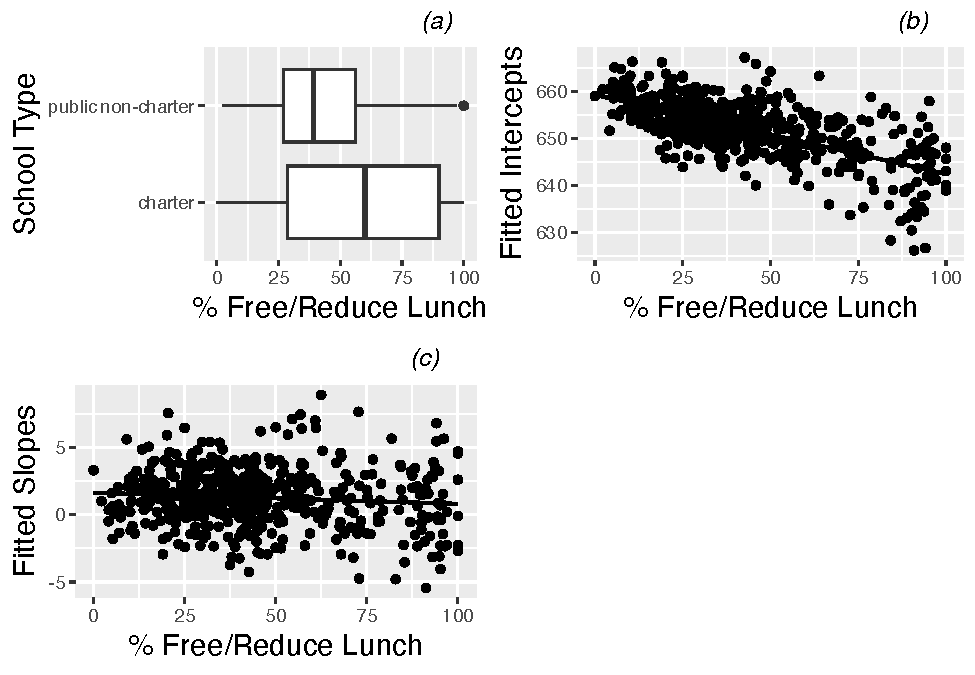
\includegraphics[width=0.6\linewidth]{bookdown-bysh_files/figure-latex/lon-boxcatmat1-1} 

}

\caption{(a) Boxplot of percent free and reduced lunch by school type (charter vs. public non-charter), along with scatterplots of (b) intercepts and (c) slopes from fitted regression lines by school vs. percent free and reduced lunch.}\label{fig:lon-boxcatmat1}
\end{figure}

\begin{figure}

{\centering 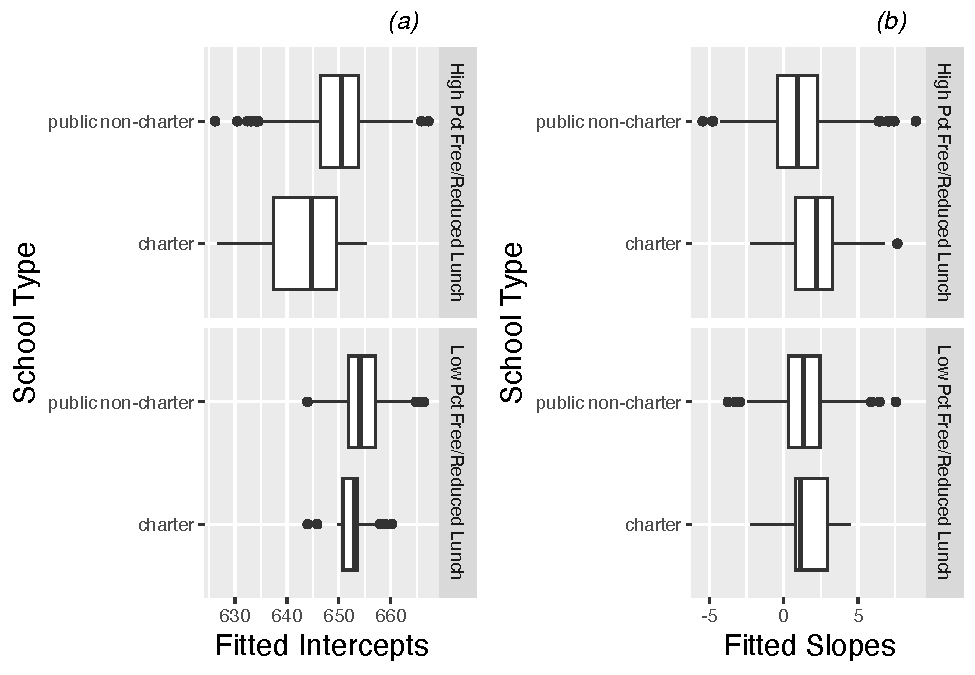
\includegraphics[width=0.6\linewidth]{bookdown-bysh_files/figure-latex/lon-boxmat1-1} 

}

\caption{Boxplots of (a) intercepts and (b) slopes from fitted regression lines by school vs. school type (charter vs. public non-charter), separated by high and low levels of percent free and reduced lunch.}\label{fig:lon-boxmat1}
\end{figure}

The effect of other confounding variables (e.g., percent non-white, percent special education, urban or rural location) can be investigated in a similar fashion to free and reduced lunch percentage, both in terms of main effect (variability in outcomes such as slope and intercept which can be explained by the confounding variable) and interaction with school type (ability of the confounding variable to explain differences between charter and public non-charter schools). We leave these explorations as an exercise.

\hypertarget{lineartwostageerror}{%
\subsection{Error structure within schools}\label{lineartwostageerror}}

Finally, with longitudinal data it is important to investigate the error variance-covariance structure of data collected within a school (the Level Two observational unit). In multilevel data, as in the examples we introduced in Chapter \ref{ch-corrdata}, we suspect observations within group (like a school) to be correlated, and we strive to model that correlation. When the data within group is collected over time, we often see distinct patterns in the residuals that can be modeled---correlations which decrease systematically as the time interval increases, variances that change over time, correlation structure that depends on a covariate, etc. A first step in modeling the error variance-covariance structure is the production of an exploratory plot such as Figure \ref{fig:lon-cor1}. To generate this plot, we begin by modeling MCA math score as a linear function of time using all 1733 observations and ignoring the school variable. This population (marginal) trend is illustrated in Figure \ref{fig:lon-spag1} and is given by:

\begin{equation}
\hat{Y}_{ij}=651.69+1.20\textstyle{Time}_{ij},
\label{eq:overalltrend}
\end{equation}
where \(\hat{Y}_{ij}\) is the predicted math score of the \(i^{th}\) school at time \(j\), where time \(j\) is the number of years since 2008. In this model, the predicted math score will be identical for all schools at a given time point \(j\). Residuals \(Y_{ij}-\hat{Y}_{ij}\) are then calculated for each observation, measuring the difference between actual math score and the average overall time trend. Figure \ref{fig:lon-cor1} then combines three pieces of information: the upper right triangle contains correlation coefficients for residuals between pairs of years, the diagonal contains histograms of residuals at each time point, and the lower left triangle contains scatterplots of residuals from two different years. In our case, we see that correlation between residuals from adjacent years is strongly positive (0.81-0.83) and does not drop off greatly as the time interval between years increases.

\begin{figure}

{\centering 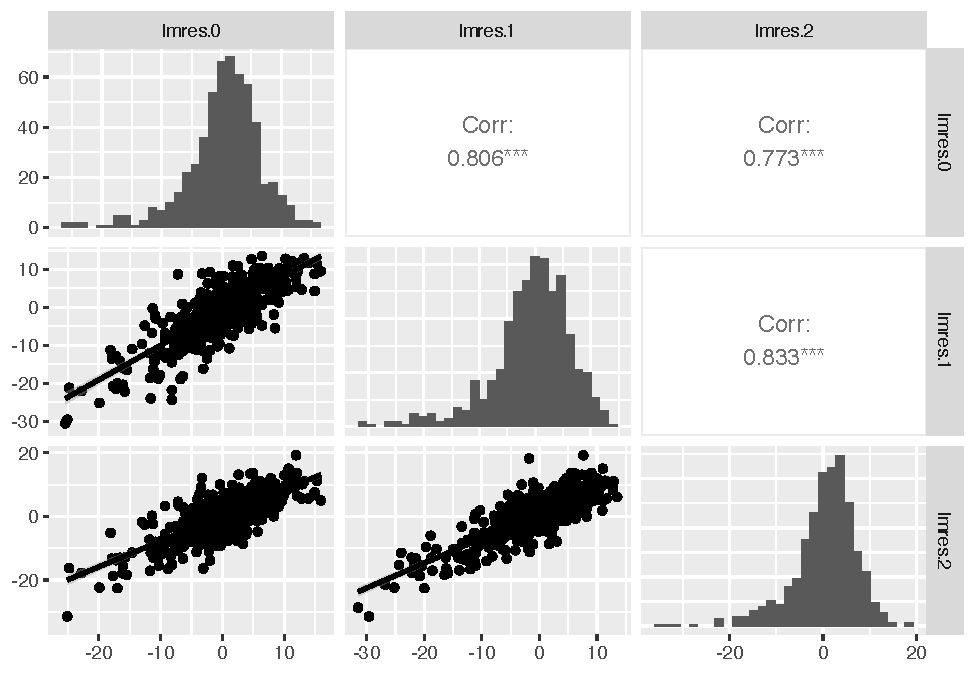
\includegraphics[width=0.6\linewidth]{bookdown-bysh_files/figure-latex/lon-cor1-1} 

}

\caption{Correlation structure within school.  The upper right contains correlation coefficients between residuals at pairs of time points, the lower left contains scatterplots of the residuals at time point pairs, and the diagonal contains histograms of residuals at each of the three time points.}\label{fig:lon-cor1}
\end{figure}

\hypertarget{lineartwostageerror}{%
\section{Initial models}\label{lineartwostageerror}}

Throughout the exploratory analysis phase, our original research questions have guided our work, and now with modeling we return to familiar questions such as:

\begin{itemize}
\tightlist
\item
  are differences between charter and public non-charter schools (in intercept, in slope, in 2010 math score) statistically significant?
\item
  are differences between school types statistically significant, even after accounting for school demographics and location?
\item
  do charter schools offer any measurable benefit over non-charter public schools, either overall or within certain subgroups of schools based on demographics or location?
\end{itemize}

As you might expect, answers to these questions will arise from proper consideration of variability and properly identified statistical models.
As in Chapter \ref{ch-multilevelintro}, we will begin model fitting with some simple, preliminary models, in part to establish a baseline for evaluating larger models. Then, we can build toward a final model for inference by attempting to add important covariates, centering certain variables, and checking assumptions.

\hypertarget{modela}{%
\subsection{Unconditional means model}\label{modela}}

In the multilevel context, we almost always begin with the \textbf{unconditional means model}, in which there are no predictors at any level. The purpose of the unconditional means model is to assess the amount of variation at each level, and to compare variability within school to variability between schools. Define \(Y_{ij}\) as the MCA-II math score from school \(i\) and year \(j\). Using the composite model specification from Chapter \ref{ch-multilevelintro}:

\begin{equation}
Y _{ij} = \alpha_{0} + u_{i} + \epsilon_{ij} \textrm{ with } u_{i} \sim N(0, \sigma^2_u) \textrm{ and } \epsilon_{ij} \sim N(0, \sigma^2)
\end{equation}
the unconditional means model can be fit to the MCA-II data:

\begin{Shaded}
\begin{Highlighting}[]
\CommentTok{#Model A (Unconditional means model)}
\NormalTok{model.a <-}\StringTok{ }\KeywordTok{lmer}\NormalTok{(MathAvgScore}\OperatorTok{~}\StringTok{ }\DecValTok{1} \OperatorTok{+}\StringTok{ }\NormalTok{(}\DecValTok{1}\OperatorTok{|}\NormalTok{schoolid), }
                \DataTypeTok{REML=}\NormalTok{T, }\DataTypeTok{data=}\NormalTok{chart.long)}
\end{Highlighting}
\end{Shaded}

\begin{verbatim}
##  Groups   Name        Variance Std.Dev.
##  schoolid (Intercept) 41.9     6.47    
##  Residual             10.6     3.25
\end{verbatim}

\begin{verbatim}
##  Number of Level Two groups =  618
\end{verbatim}

\begin{verbatim}
##             Estimate Std. Error t value
## (Intercept)    652.7     0.2726    2395
\end{verbatim}

From this output, we obtain estimates of our three model parameters:

\begin{itemize}
\item
  \(\hat{\alpha}_{0}\) = 652.7 = the mean math score across all schools and all years
\item
  \(\hat{\sigma}^2\)= 10.6 = the variance in within-school deviations between individual scores and the school mean across all years
\item
  \(\hat{\sigma}^2_u\)= 41.9 = the variance in between-school deviations between school means and the overall mean across all schools and all years
\end{itemize}

Based on the intraclass correlation coefficient:

\begin{equation}
\hat{\rho}=\frac{\hat{\sigma}^2_u}{\hat{\sigma}^2_u + \hat{\sigma}^2} = \frac{41.869}{41.869+10.571}= 0.798
\end{equation}
79.8 percent of the total variation in math scores is attributable to difference among schools rather than changes over time within schools. We can also say that the average correlation for any pair of responses from the same school is 0.798.

\hypertarget{modelb}{%
\subsection{Unconditional growth model}\label{modelb}}

The second model in most multilevel contexts introduces a covariate at Level One (see Model B in Chapter \ref{ch-multilevelintro}). With longitudinal data, this second model introduces time as a predictor at Level One, but there are still no predictors at Level Two. This model is then called the \textbf{unconditional growth model}. The unconditional growth model allows us to assess how much of the within-school variability can be attributed to systematic changes over time.

At the lowest level, we can consider building individual growth models over time for each of the 618 schools in our study. First, we must decide upon a form for each of our 618 growth curves. Based on our initial exploratory analyses, assuming that an individual school's MCA-II math scores follow a linear trend seems like a reasonable starting point. Under the assumption of linearity, we must estimate an intercept and a slope for each school, based on their 1-3 test scores over a period of three years. Compared to time series analyses of economic data, most longitudinal data analyses have relatively few time periods for each subject (or school), and the basic patterns within subject are often reasonably described by simpler functional forms.

Let \(Y_{ij}\) be the math score of the \(i^{th}\) school in year \(j\). Then we can model the linear change in math test scores over time for School \(i\) according to Model B:

\begin{equation}
Y_{ij} = a_{i} + b_{i}Year08_{ij} + \epsilon_{ij} \textrm{ where } \epsilon_{ij} \sim N(0, \sigma^2)
\end{equation}

The parameters in this model \((a_{i}, b_{i},\) and \(\sigma^2)\) can be estimated through LLSR methods. \(a_{i}\) represents the true intercept for School \(i\)---i.e., the expected test score level for School \(i\) when time is zero (2008)---while \(b_{i}\) represents the true slope for School \(i\)---i.e., the expected yearly rate of change in math score for School \(i\) over the three year observation period. Here we use Roman letters rather than Greek for model parameters since models by school will eventually be a conceptual first step in a multilevel model. The \(\epsilon_{ij}\) terms represent the deviation of School \(i\)'s actual test scores from the expected results under linear growth---the part of school \(i\)'s test score at time \(j\) that is not explained by linear changes over time. The variability in these deviations from the linear model is given by \(\sigma^2\). In Figure \ref{fig:lon-scat3}, which illustrates a linear growth model for Norwood Central Middle School, \(a_{i}\) is estimated by the \(y\)-intercept of the fitted regression line, \(b_{i}\) is estimated by the slope of the fitted regression line, and \(\sigma^2\) is estimated by the variability in the vertical distances between each point (the actual math score in year \(j\)) and the line (the predicted math score in year \(j\)).

\begin{verbatim}
## `geom_smooth()` using formula 'y ~ x'
\end{verbatim}

\begin{figure}

{\centering 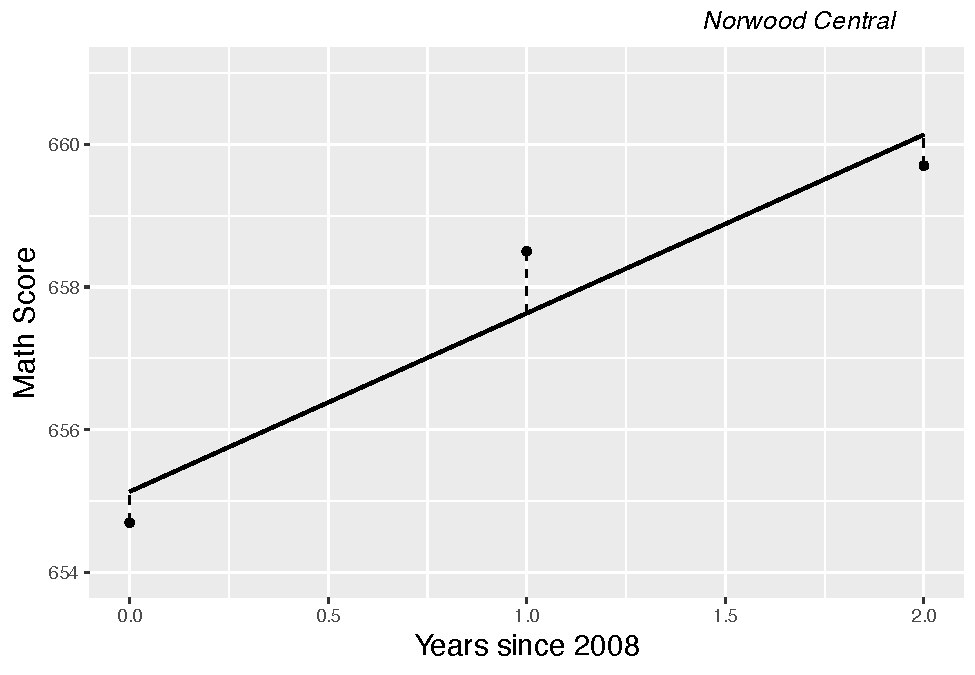
\includegraphics[width=0.6\linewidth]{bookdown-bysh_files/figure-latex/lon-scat3-1} 

}

\caption{Linear growth model for Norwood Central Middle School}\label{fig:lon-scat3}
\end{figure}

In a multilevel model, we let intercepts (\(a_{i}\)) and slopes (\(b_{i}\)) vary by school and build models for these intercepts and slopes using school-level variables at Level Two. An unconditional growth model features no predictors at Level Two and can be specified either using formulations at both levels:

\begin{itemize}
\item
  Level One:
  \begin{equation}
  Y_{ij}=a_{i}+b_{i}Year08_{ij} + \epsilon_{ij}
  \end{equation}
\item
  Level Two:
  \begin{align*}
  a_{i}&=\alpha_{0} + u_{i}\\
  b_{i}&=\beta_{0} + v_{i}
  \end{align*}
\end{itemize}

or as a composite model:

\begin{equation}
Y_{ij}=\alpha_{0} + \beta_{0}Year08_{ij}+u_{i}+v_{i}Year08_{ij} + \epsilon_{ij}
\end{equation}
where \(\epsilon_{ij}\sim N(0,\sigma^2)\) and

\[ \left[ \begin{array}{c}
            u_{i} \\ v_{i}
          \end{array}  \right] \sim N \left( \left[
          \begin{array}{c}
            0 \\ 0
          \end{array} \right], \left[
          \begin{array}{cc}
            \sigma_{u}^{2} & \\
            \sigma_{uv} & \sigma_{v}^{2}
          \end{array} \right] \right) . \]

As before, \(\sigma^2\) quantifies the within-school variability (the scatter of points around schools' linear growth trajectories), while now the between-school variability is partitioned into variability in initial status \((\sigma^2_u)\) and variability in rates of change \((\sigma^2_v)\).

Using the composite model specification, the unconditional growth model can be fit to the MCA-II test data:

\begin{Shaded}
\begin{Highlighting}[]
\CommentTok{#Model B (Unconditional growth)}
\NormalTok{model.b <-}\StringTok{ }\KeywordTok{lmer}\NormalTok{(MathAvgScore}\OperatorTok{~}\StringTok{ }\NormalTok{year08 }\OperatorTok{+}\StringTok{ }\NormalTok{(year08}\OperatorTok{|}\NormalTok{schoolid), }
  \DataTypeTok{REML=}\NormalTok{T, }\DataTypeTok{data=}\NormalTok{chart.long)}
\end{Highlighting}
\end{Shaded}

\begin{verbatim}
##  Groups   Name        Variance Std.Dev. Corr
##  schoolid (Intercept) 39.441   6.280        
##           year08       0.111   0.332    0.72
##  Residual              8.820   2.970
\end{verbatim}

\begin{verbatim}
##  Number of Level Two groups =  618
\end{verbatim}

\begin{verbatim}
##             Estimate Std. Error t value
## (Intercept)  651.408    0.27934 2331.96
## year08         1.265    0.08997   14.06
\end{verbatim}

\begin{verbatim}
##  AIC =  10352 ;  BIC =  10384
\end{verbatim}

From this output, we obtain estimates of our six model parameters:

\begin{itemize}
\tightlist
\item
  \(\hat{\alpha}_{0}\) = 651.4 = the mean math score for the population of schools in 2008.
\item
  \(\hat{\beta}_{0}\) = 1.26 = the mean yearly change in math test scores for the population during the three year observation period.
\item
  \(\hat{\sigma}^2\) = 8.82 = the variance in within-school deviations.
\item
  \(\hat{\sigma}^2_u\) = 39.4 = the variance between schools in 2008 scores.
\item
  \(\hat{\sigma}^2_v\) = 0.11 = the variance between schools in rates of change in math test scores during the three year observation period.
\item
  \(\hat{\rho}_{uv}\) = 0.72 = the correlation in schools' 2008 math score and their rate of change in scores between 2008 and 2010.
\end{itemize}

We see that schools had a mean math test score of 651.4 in 2008 and their mean test scores tended to increase by 1.26 points per year over the three year observation period, producing a mean test score at the end of three years of 653.9. According to the t-value (14.1), the increase in mean test scores noted during the three year observation period is statistically significant.

The estimated within-school variance \(\hat{\sigma}^2\) decreased by about 17\% from the unconditional means model, implying that 17\% of within-school variability in test scores can be explained by a linear increase over time:

\begin{align*}
\textrm{Pseudo }R^2_{L1} & = \frac{\hat{\sigma}^2(\textrm{uncond means}) - \hat{\sigma}^2(\textrm{uncond growth})}{\hat{\sigma^2}(\textrm{uncond means})} \\
 & = \frac{10.571-8.820}{10.571}= 0.17
\end{align*}

\hypertarget{othertimetrends}{%
\subsection{Modeling other trends over time}\label{othertimetrends}}

While modeling linear trends over time is often a good approximation of reality, it is by no means the only way to model the effect of time. One alternative is to model the quadratic effect of time, which implies adding terms for both time and the square of time. Typically, to reduce the correlation between the linear and quadratic components of the time effect, the time variable is often centered first; we have already ``centered'' on 2008. Modifying Model B to produce an \textbf{unconditional quadratic growth model} would take the following form:

\begin{itemize}
\item
  Level One:
  \begin{equation}
  Y_{ij}=a_{i}+b_{i}Year08_{ij}+c_{i}Year08^{2}_{ij} + \epsilon_{ij}
  \end{equation}
\item
  Level Two:
  \begin{align*}
  a_{i} & = \alpha_{0} + u_{i}\\
  b_{i} & = \beta_{0} + v_{i}\\
  c_{i} & = \gamma_{0} + w_{i}
  \end{align*}
  where \(\epsilon_{ij}\sim N(0,\sigma^2)\) and
\end{itemize}

\[ \left[ \begin{array}{c}
            u_{i} \\ v_{i} \\ w_{i}
          \end{array}  \right] \sim N \left( \left[
          \begin{array}{c}
            0 \\ 0 \\ 0
          \end{array} \right], \left[
          \begin{array}{ccc}
            \sigma_{u}^{2} & & \\
            \sigma_{uv} & \sigma_{v}^{2} & \\
            \sigma_{uw} & \sigma_{vw} & \sigma_{w}^{2}
          \end{array} \right] \right) . \]

With the extra term at Level One for the quadratic effect, we now have 3 equations at Level Two, and 6 variance components at Level Two (3 variance terms and 3 covariance terms). However, with only a maximum of 3 observations per school, we lack the data for fitting 3 equations with error terms at Level Two. Instead, we could model the quadratic time effect with fewer variance components---for instance, by only using an error term on the intercept at Level Two:\\
\begin{align*}
a_{i} & = \alpha_{0} + u_{i}\\
b_{i} & = \beta_{0}\\ 
c_{i} & = \gamma_{0}
\end{align*}
where \(u_{i}\sim N(0,\sigma^2_u)\). Models like this are frequently used in practice---they allow for a separate overall effect on test scores for each school while minimizing parameters that must be estimated. The tradeoff is that this model does not allow linear and quadratic effects to differ by school, but we have little choice here without more observations per school. Thus, using the composite model specification, the unconditional quadratic growth model with random intercept for each school can be fit to the MCA-II test data:

\begin{Shaded}
\begin{Highlighting}[]
\CommentTok{# Modeling quadratic time trend}
\NormalTok{model.b2 <-}\StringTok{ }\KeywordTok{lmer}\NormalTok{(MathAvgScore}\OperatorTok{~}\StringTok{ }\NormalTok{yearc }\OperatorTok{+}\StringTok{ }\NormalTok{yearc2 }\OperatorTok{+}\StringTok{ }\NormalTok{(}\DecValTok{1}\OperatorTok{|}\NormalTok{schoolid), }
  \DataTypeTok{REML=}\NormalTok{T, }\DataTypeTok{data=}\NormalTok{chart.long)}
\end{Highlighting}
\end{Shaded}

\begin{verbatim}
##  Groups   Name        Variance Std.Dev.
##  schoolid (Intercept) 43.05    6.56    
##  Residual              8.52    2.92
\end{verbatim}

\begin{verbatim}
##  Number of Level Two groups =  618
\end{verbatim}

\begin{verbatim}
##             Estimate Std. Error  t value
## (Intercept)  651.942    0.29229 2230.448
## yearc          1.270    0.08758   14.501
## yearc2         1.068    0.15046    7.101
\end{verbatim}

\begin{verbatim}
##  AIC =  10308 ;  BIC =  10335
\end{verbatim}

From this output, we see that the quadratic effect is positive and significant (t=7.1), in this case indicating that increases in test scores are greater between 2009 and 2010 than between 2008 and 2009. Based on AIC and BIC values, the quadratic growth model outperforms the linear growth model with random intercepts only at level Two (AIC: 10308 vs.~10354; BIC: 10335 vs.~10375).

Another frequently used approach to modeling time effects is the \textbf{piecewise linear model}. In this model, the complete time span of the study is divided into two or more segments, with a separate slope relating time to the response in each segment. In our case study there is only one piecewise option---fitting separate slopes in 2008-09 and 2009-10. With only 3 time points, creating a piecewise linear model is a bit simplified, but this idea can be generalized to segments with more than two years each.

The performance of this model is very similar to the quadratic growth model by AIC and BIC measures, and the story told by fixed effects estimates is also very similar. While the mean yearly increase in math scores was 0.2 points between 2008 and 2009, it was 2.3 points between 2009 and 2010.

Despite the good performances of the quadratic growth and piecewise linear models on our three-year window of data, we will continue to use linear growth assumptions in the remainder of this chapter. Not only is a linear model easier to interpret and explain, but it's probably a more reasonable assumption in years beyond 2010. Predicting future performance is more risky by assuming a steep one year rise or a non-linear rise will continue, rather than by using the average increase over two years.

\hypertarget{finalmodel}{%
\section{Building to a final model}\label{finalmodel}}

\hypertarget{sec:modelc9}{%
\subsection{Uncontrolled effects of school type}\label{sec:modelc9}}

Initially, we can consider whether or not there are significant differences in individual school growth parameters (intercepts and slopes) based on school type. From a modeling perspective, we would build a system of two Level Two models:

\begin{align*}
a_{i} & = \alpha_{0} + \alpha_{1}Charter_i + u_{i} \\
b_{i} & = \beta_{0} + \beta_{1}Charter_i + v_{i}
\end{align*}
where \(Charter_i=1\) if School \(i\) is a charter school and \(Charter_i=0\) if School \(i\) is a non-charter public school. In addition, the error terms at Level Two are assumed to follow a multivariate normal distribution:

\[ \left[ \begin{array}{c}
            u_{i} \\ v_{i}
          \end{array}  \right] \sim N \left( \left[
          \begin{array}{c}
            0 \\ 0
          \end{array} \right], \left[
          \begin{array}{cc}
            \sigma_{u}^{2} & \\
            \sigma_{uv} & \sigma_{v}^{2}
          \end{array} \right] \right) . \]

With a binary predictor at Level Two such as school type, we can write out what our Level Two model looks like for public non-charter schools and charter schools.

\begin{itemize}
\tightlist
\item
  Public schools
\end{itemize}

\begin{align*}
a_{i} & = \alpha_{0} + u_{i}\\
b_{i} & = \beta_{0} + v_{i},
\end{align*}

\begin{itemize}
\tightlist
\item
  Charter schools
\end{itemize}

\begin{align*}
a_{i} & = (\alpha_{0} + \alpha_{1}) + u_{i}\\
b_{i} & = (\beta_{0}+ \beta_{1}) + v_{i}
\end{align*}

Writing the Level Two model in this manner helps us interpret the model parameters from our two-level model. We can use statistical software (such as the lmer() function from the lme4 package in R) to obtain parameter estimates using our \(1733\) observations, after first converting our Level One and Level Two models into a composite model (Model C) with fixed effects and variance components separated:

\begin{align*}
Y_{ij} & = a_{i} + b_{i}Year08_{ij}+ \epsilon_{ij} \\
       & = (\alpha_{0} + \alpha_{1}Charter_i +u_{i}) + (\beta_{0} + \beta_{1}Charter_i + v_{i})Year08_{ij} + \epsilon_{ij} \\
       & = [\alpha_{0} + \beta_{0}Year08_{ij} +\alpha_{1}Charter_i+ \beta_{1}Charter_iYear08_{ij}] + \\
       & \quad [u_{i} + v_{i}Year08_{ij} + \epsilon_{ij}]
\end{align*}

\begin{Shaded}
\begin{Highlighting}[]
\CommentTok{#Model C (uncontrolled effects of school type on }
\CommentTok{#   intercept and slope)}
\NormalTok{model.c <-}\StringTok{ }\KeywordTok{lmer}\NormalTok{(MathAvgScore}\OperatorTok{~}\StringTok{ }\NormalTok{charter }\OperatorTok{+}\StringTok{ }\NormalTok{year08 }\OperatorTok{+}\StringTok{ }
\StringTok{  }\NormalTok{charter}\OperatorTok{:}\NormalTok{year08 }\OperatorTok{+}\StringTok{ }\NormalTok{(year08}\OperatorTok{|}\NormalTok{schoolid), }
  \DataTypeTok{REML=}\NormalTok{T, }\DataTypeTok{data=}\NormalTok{chart.long)}
\end{Highlighting}
\end{Shaded}

\begin{verbatim}
##  Groups   Name        Variance Std.Dev. Corr
##  schoolid (Intercept) 35.832   5.986        
##           year08       0.131   0.362    0.88
##  Residual              8.784   2.964
\end{verbatim}

\begin{verbatim}
##  Number of Level Two groups =  618
\end{verbatim}

\begin{verbatim}
##                Estimate Std. Error  t value
## (Intercept)    652.0584    0.28449 2291.996
## charter         -6.0184    0.86562   -6.953
## year08           1.1971    0.09427   12.698
## charter:year08   0.8557    0.31430    2.723
\end{verbatim}

\begin{verbatim}
##  AIC =  10308 ;  BIC =  10351
\end{verbatim}

Armed with our parameter estimates, we can offer concrete interpretations:

\begin{itemize}
\item
  Fixed effects:

  \begin{itemize}
  \tightlist
  \item
    \(\hat{\alpha}_{0} = 652.1.\) The estimated mean test score for 2008 for non-charter public schools is 652.1.
  \item
    \(\hat{\alpha}_{1}= -6.02.\) Charter schools have an estimated test score in 2008 which is 6.02 points lower than public non-charter schools.
  \item
    \(\hat{\beta}_{0}= 1.20.\) Public non-charter schools have an estimated mean increase in test scores of 1.20 points per year.
  \item
    \(\hat{\beta}_{1}= 0.86.\) Charter schools have an estimated mean increase in test scores of 2.06 points per year over the three year observation period, 0.86 points higher than the mean yearly increase among public non-charter schools.
  \end{itemize}
\item
  Variance components:

  \begin{itemize}
  \tightlist
  \item
    \(\hat{\sigma}_u= 5.99.\) The estimated standard deviation of 2008 test scores is 5.99 points, after controlling for school type.
  \item
    \(\hat{\sigma}_v= 0.36.\) The estimated standard deviation of yearly changes in test scores during the three year observation period is 0.36 points, after controlling for school type.
  \item
    \(\hat{\rho}_{uv}= 0.88.\) The estimated correlation between 2008 test scores and yearly changes in test scores is 0.88, after controlling for school type.
  \item
    \(\hat{\sigma}= 2.96.\) The estimated standard deviation in residuals for the individual growth curves is 2.96 points.
  \end{itemize}
\end{itemize}

Based on t-values reported by R, the effects of \texttt{year08} and \texttt{charter} both appear to be statistically significant, and there is also significant evidence of an interaction between \texttt{year08} and \texttt{charter}. Public schools had a significantly higher mean math score in 2008, while charter schools had significantly greater improvement in scores between 2008 and 2010 (although the mean score of charter schools still lagged behind that of public schools in 2010, as indicated in the graphical comparison of models B and C in Figure \ref{fig:lon-scat4}). Based on pseudo R-square values, the addition of a charter school indicator to the unconditional growth model has decreased unexplained school-to-school variability in 2008 math scores by 4.7\%, while unexplained variability in yearly improvement actually increased slightly. Obviously, it makes little sense that introducing an additional predictor would \emph{reduce} the amount of variability in test scores explained, but this is an example of the limitations in the pseudo \(R^2\) values discussed in Section \ref{pseudoR2}.

\begin{figure}

{\centering 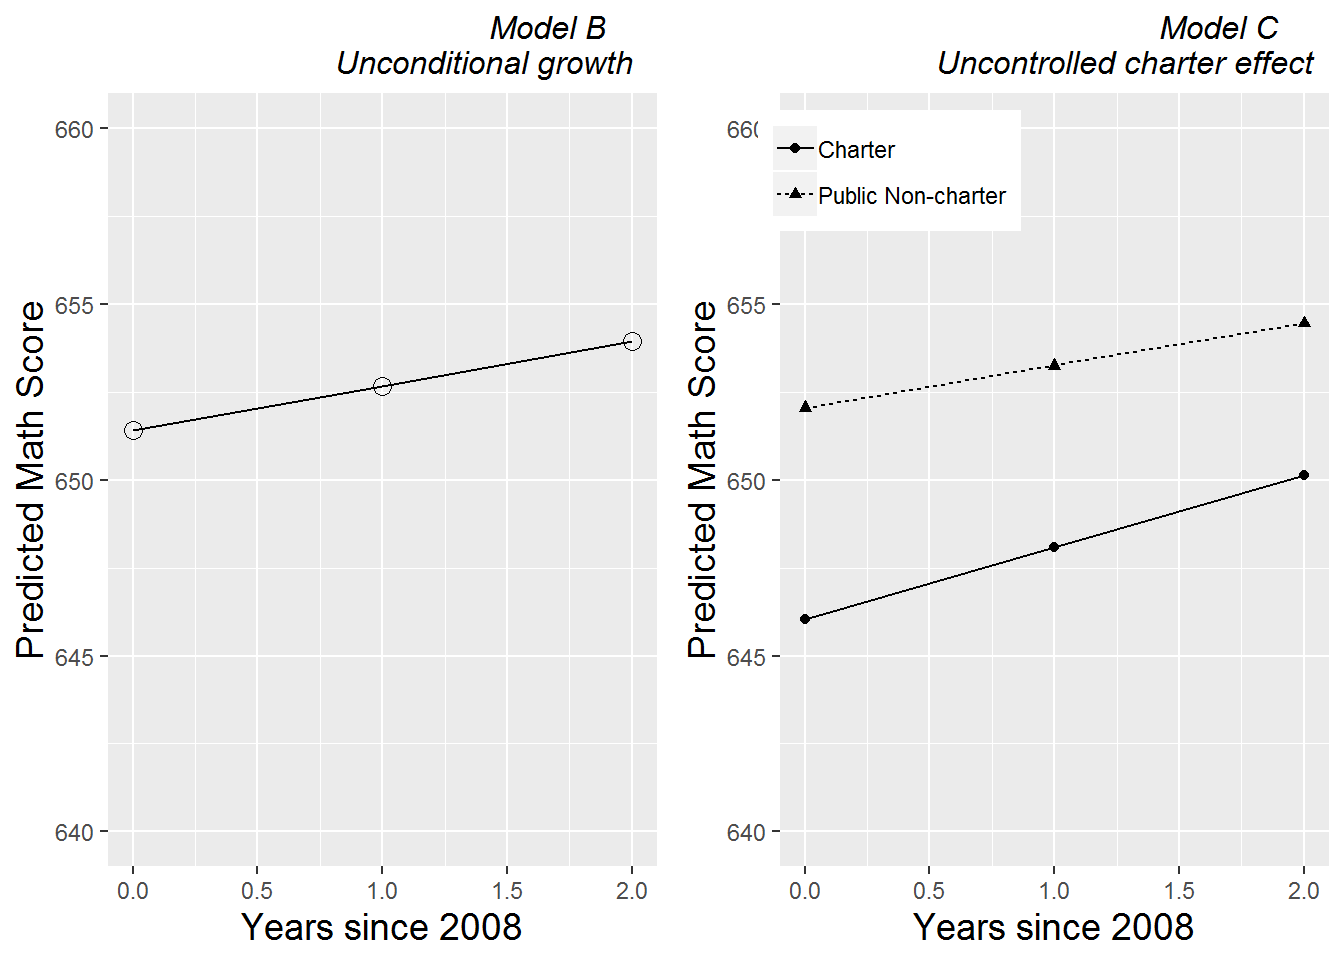
\includegraphics[width=0.6\linewidth]{bookdown-bysh_files/figure-latex/lon-scat4-1} 

}

\caption{ Fitted growth curves for Models B and C.}\label{fig:lon-scat4}
\end{figure}

\hypertarget{modeld}{%
\subsection{Add percent free and reduced lunch as a covariate}\label{modeld}}

Although we will still be primarily interested in the effect of school type on both 2008 test scores and rate of change in test scores (as we observed in Model C), we can try to improve our estimates of school type effects through the introduction of meaningful covariates. In this study, we are particularly interested in Level Two covariates---those variables which differ by school but which remain basically constant for a given school over time---such as urban or rural location, percentage of special education students, and percentage of students with free and reduced lunch. In Section \ref{twostage9}, we investigated the relationship between percent free and reduced lunch and a school's test score in 2008 and their rate of change from 2008 to 2010.

Based on these analyses, we will begin by adding percent free and reduced lunch as a Level Two predictor for both intercept and slope (Model D):

\begin{itemize}
\item
  Level One:
  \begin{equation}
  Y_{ij}=a_{i} + b_{i}Year08_{ij} + \epsilon_{ij}
  \end{equation}
\item
  Level Two:
  \begin{align*}
  a_{i} & = \alpha_{0} + \alpha_{1}Charter_i + \alpha_{2}schpctfree_i + u_{i}\\
  b_{i} & = \beta_{0} + \beta_{1}Charter_i + \beta_{2}schpctfree_i + v_{i}
  \end{align*}
\end{itemize}

The composite model is then:

\begin{align}
Y_{ij}= [\alpha_{0}&+\alpha_{1}Charter_i +\alpha_{2}schpctfree_i + \beta_{0}Year08_{ij} \nonumber \\
 &+ \beta_{1}Charter_iYear08_{ij}  + \beta_{2}schpctfree_iYear08_{ij}] \nonumber \\ 
 &+ [u_{i} + v_{i}Year08_{ij} + \epsilon_{ij}]
\end{align}
where error terms are defined as in Model C.

\begin{Shaded}
\begin{Highlighting}[]
\CommentTok{#Model D2 (Introduce SchPctFree at level 2)}
\NormalTok{model.d2 <-}\StringTok{ }\KeywordTok{lmer}\NormalTok{(MathAvgScore}\OperatorTok{~}\StringTok{ }\NormalTok{charter }\OperatorTok{+}\StringTok{ }\NormalTok{SchPctFree }\OperatorTok{+}\StringTok{ }\NormalTok{year08 }\OperatorTok{+}\StringTok{ }
\StringTok{  }\NormalTok{charter}\OperatorTok{:}\NormalTok{year08 }\OperatorTok{+}\StringTok{ }\NormalTok{SchPctFree}\OperatorTok{:}\NormalTok{year08 }\OperatorTok{+}\StringTok{ }\NormalTok{(year08}\OperatorTok{|}\NormalTok{schoolid),}
  \DataTypeTok{REML=}\NormalTok{T, }\DataTypeTok{data=}\NormalTok{chart.long)}
\end{Highlighting}
\end{Shaded}

\begin{verbatim}
##  Groups   Name        Variance Std.Dev. Corr
##  schoolid (Intercept) 19.13    4.37         
##           year08       0.16    0.40     0.51
##  Residual              8.80    2.97
\end{verbatim}

\begin{verbatim}
##  Number of Level Two groups =  618
\end{verbatim}

\begin{verbatim}
##                    Estimate Std. Error  t value
## (Intercept)       659.27848   0.444690 1482.558
## charter            -3.43994   0.712836   -4.826
## SchPctFree         -0.16654   0.008907  -18.697
## year08              1.64137   0.189499    8.662
## charter:year08      0.98076   0.318583    3.078
## SchPctFree:year08  -0.01041   0.003839   -2.711
\end{verbatim}

\begin{verbatim}
##  AIC =  9988 ;  BIC =  10043
\end{verbatim}

\begin{Shaded}
\begin{Highlighting}[]
\NormalTok{drop_in_dev <-}\StringTok{ }\KeywordTok{anova}\NormalTok{(model.d2, model.c, }\DataTypeTok{test =} \StringTok{"Chisq"}\NormalTok{)}
\end{Highlighting}
\end{Shaded}

\begin{verbatim}
         npar   AIC   BIC logLik   dev Chisq Df
model.c     8 10305 10348  -5144 10289    NA NA
model.d2   10  9967 10022  -4974  9947 341.5  2
              pval
model.c         NA
model.d2 7.158e-75
\end{verbatim}

Compared to Model C, the introduction of school-level poverty based on percentage of students receiving free and reduced lunch in Model D leads to similar conclusions about the significance of the charter school effect on both the intercept and the slope, although the magnitude of these estimates change after controlling for poverty levels. The estimated gap in test scores between charter and non-charter schools in 2008 is smaller in Model D, while estimates of improvement between 2008 and 2010 increase for both types of schools. Inclusion of free and reduced lunch reduces the unexplained variability between schools in 2008 math scores by 27\%, while unexplained variability in rates of change between schools again increases slightly based on pseudo \(R^2\) values. A \textbf{likelihood ratio test} using maximum likelihood estimates illustrates that adding free and reduced lunch as a Level Two covariate significantly improves our model (\(\chi^2 = 341.5, df=2, p<.001\)). Specific fixed effect parameter estimates are given below:

\begin{itemize}
\item
  \(\hat{\alpha}_{0}= 659.3.\) The estimated mean math test score for 2008 is 659.3 for non-charter public schools with no students receiving free and reduced lunch.
\item
  \(\hat{\alpha}_{1}= -3.44.\) Charter schools have an estimated mean math test score in 2008 which is 3.44 points lower than non-charter public schools, controlling for effects of school-level poverty.
\item
  \(\hat{\alpha}_{2}= -0.17.\) Each 10\% increase in the percentage of students at a school receiving free and reduced lunch is associated with a 1.7 point decrease in mean math test scores for 2008, after controlling for school type.
\item
  \(\hat{\beta}_{0}= 1.64.\) Public non-charter schools with no students receiving free and reduced lunch have an estimated mean increase in math test score of 1.64 points per year during the three years of observation.
\item
  \(\hat{\beta}_{1}= 0.98.\) Charter schools have an estimated mean yearly increase in math test scores over the three year observation period of 2.62, which is 0.98 points higher than the annual increase for public non-charter schools, after controlling for school-level poverty.
\item
  \(\hat{\beta}_{2}= -0.010.\) Each 10\% increase in the percentage of students at a school receiving free and reduced lunch is associated with a 0.10 point decrease in rate of change over the three years of observation, after controlling for school type.
\end{itemize}

\hypertarget{modelf9}{%
\subsection{A potential final model with three Level Two covariates}\label{modelf9}}

We now begin iterating toward a ``final model'' for these data, on which we will base conclusions. Being cognizant of typical features of a ``final model'' as outlined in Chapter \ref{ch-multilevelintro}, we offer one possible final model for this data---Model F:

\begin{itemize}
\tightlist
\item
  Level One:
\end{itemize}

\begin{equation}
Y_{ij}= a_{i} + b_{i}Year08_{ij} + \epsilon_{ij}
\end{equation}

\begin{itemize}
\tightlist
\item
  Level Two:
\end{itemize}

\begin{align*}
a_{i} & = \alpha_{0} + \alpha_{1}Charter_i + \alpha_{2}urban_i + \alpha_{3}schpctsped_i + \alpha_{4}schpctfree_i + u_{i} \\
b_{i} & = \beta_{0} + \beta_{1}Charter_i + \beta_{2}urban_i + \beta_{3}schpctsped_i + v_{i}
\end{align*}

where we find the effect of charter schools on 2008 test scores after adjusting for urban or rural location, percentage of special education students, and percentage of students that receive free or reduced lunch, and the effect of charter schools on yearly change between 2008 and 2010 after adjusting for urban or rural location and percentage of special education students. We can use AIC and BIC criteria to compare Model F with Model D, since the two models are not nested. By both criteria, Model F is significantly better than Model D: AIC of 9855 vs.~9988, and BIC of 9956 vs.~10043. Based on the R output below, we offer interpretations for estimates of model fixed effects:

\begin{Shaded}
\begin{Highlighting}[]
\NormalTok{model.f2 <-}\StringTok{ }\KeywordTok{lmer}\NormalTok{(MathAvgScore }\OperatorTok{~}\StringTok{ }\NormalTok{charter }\OperatorTok{+}\StringTok{ }\NormalTok{urban }\OperatorTok{+}\StringTok{ }\NormalTok{SchPctFree }\OperatorTok{+}\StringTok{ }
\StringTok{  }\NormalTok{SchPctSped }\OperatorTok{+}\StringTok{ }\NormalTok{charter}\OperatorTok{:}\NormalTok{year08 }\OperatorTok{+}\StringTok{ }\NormalTok{urban}\OperatorTok{:}\NormalTok{year08 }\OperatorTok{+}\StringTok{ }
\StringTok{  }\NormalTok{SchPctSped}\OperatorTok{:}\NormalTok{year08 }\OperatorTok{+}\StringTok{ }\NormalTok{year08 }\OperatorTok{+}
\StringTok{  }\NormalTok{(year08}\OperatorTok{|}\NormalTok{schoolid), }\DataTypeTok{REML=}\NormalTok{T, }\DataTypeTok{data=}\NormalTok{chart.long)}
\end{Highlighting}
\end{Shaded}

\begin{verbatim}
##  Groups   Name        Variance Std.Dev. Corr
##  schoolid (Intercept) 16.94756 4.1167       
##           year08       0.00475 0.0689   0.85
##  Residual              8.82197 2.9702
\end{verbatim}

\begin{verbatim}
##  Number of Level Two groups =  618
\end{verbatim}

\begin{verbatim}
##                    Estimate Std. Error  t value
## (Intercept)       661.01042   0.512888 1288.800
## charter            -3.22286   0.698547   -4.614
## urban              -1.11383   0.427566   -2.605
## SchPctFree         -0.15281   0.008096  -18.874
## SchPctSped         -0.11770   0.020612   -5.710
## year08              2.14430   0.200867   10.675
## charter:year08      1.03087   0.315159    3.271
## urban:year08       -0.52749   0.186480   -2.829
## SchPctSped:year08  -0.04674   0.010166   -4.598
\end{verbatim}

\begin{verbatim}
##  AIC =  9885 ;  BIC =  9956
\end{verbatim}

\begin{itemize}
\tightlist
\item
  \(\hat{\alpha}_{0}= 661.0.\) The estimated mean math test score for 2008 is 661.0 for public schools in rural areas with no students qualifying for special education or free and reduced lunch.
\item
  \(\hat{\alpha}_{1}= -3.22.\) Charter schools have an estimated mean math test score in 2008 which is 3.22 points lower than non-charter public schools, after controlling for urban or rural location, percent special education, and percent free and reduced lunch.
\item
  \(\hat{\alpha}_{2}= -1.11.\) Schools in urban areas have an estimated mean math score in 2008 which is 1.11 points lower than schools in rural areas, after controlling for school type, percent special education, and percent free and reduced lunch.
\item
  \(\hat{\alpha}_{3}= -0.118.\) A 10\% increase in special education students at a school is associated with a 1.18 point decrease in estimated mean math score for 2008, after controlling for school type, urban or rural location, and percent free and reduced lunch.
\item
  \(\hat{\alpha}_{4}= -0.153.\) A 10\% increase in free and reduced lunch students at a school is associated with a 1.53 point decrease in estimated mean math score for 2008, after controlling for school type, urban or rural location, and percent special education.
\item
  \(\hat{\beta}_{0}= 2.14.\) Public non-charter schools in rural areas with no students qualifying for special education have an estimated increase in mean math test score of 2.14 points per year over the three year observation period, after controlling for percent of students receiving free and reduced lunch.
\item
  \(\hat{\beta}_{1}= 1.03.\) Charter schools have an estimated mean annual increase in math score that is 1.03 points higher than public non-charter schools over the three year observation period, after controlling for urban or rural location, percent special education, and percent free and reduced lunch.
\item
  \(\hat{\beta}_{2}= -0.53.\) Schools in urban areas have an estimated mean annual increase in math score that is 0.53 points lower than schools from rural areas over the three year observation period, after controlling for school type, percent special education, and percent free and reduced lunch.
\item
  \(\hat{\beta}_{3}= -0.047.\) A 10\% increase in special education students at a school is associated with an estimated mean annual increase in math score that is 0.47 points lower over the three year observation period, after controlling for school type, urban or rural location, and percent free and reduced lunch.
\end{itemize}

From this model, we again see that 2008 sixth grade math test scores from charter schools were significantly lower than similar scores from public non-charter schools, after controlling for school location and demographics. However, charter schools showed significantly greater improvement between 2008 and 2010 compared to public non-charter schools, although charter school test scores were still lower than public school scores in 2010, on average. We also tested several interactions between Level Two covariates and charter schools and found none to be significant, indicating that the 2008 gap between charter schools and public non-charter schools was consistent across demographic subgroups. The faster improvement between 2008 and 2010 for charter schools was also consistent across demographic subgroups (found by testing three-way interactions). Controlling for school location and demographic variables provided more reliable and nuanced estimates of the effects of charter schools, while also providing interesting insights. For example, schools in rural areas not only had higher test scores than schools in urban areas in 2008, but the gap grew larger over the study period given fixed levels of percent special education, percent free and reduced lunch, and school type. In addition, schools with higher levels of poverty lagged behind other schools and showed no signs of closing the gap, and schools with higher levels of special education students had both lower test scores in 2008 and slower rates of improvement during the study period, again given fixed levels of other covariates.

As we demonstrated in this case study, applying multilevel methods to two-level longitudinal data yields valuable insights about our original research questions while properly accounting for the structure of the data.

\hypertarget{errorcovariance}{%
\section{Covariance structure among observations}\label{errorcovariance}}

Part of our motivation for framing our model for multilevel data was to account for the correlation among observations made on the same school (the Level Two observational unit). Our two-level model, through error terms on both Level One and Level Two variables, actually implies a specific within-school covariance structure among observations, yet we have not (until now) focused on this imposed structure. For example:

\begin{itemize}
\tightlist
\item
  What does our two-level model say about the relative variability of 2008 and 2010 scores from the same school?
\item
  What does it say about the correlation between 2008 and 2009 scores from the same school?
\end{itemize}

In this section, we will describe the within-school covariance structure imposed by our two-level model and offer alternative covariance structures that we might consider, especially in the context of longitudinal data. In short, we will discuss how we might decide if our implicit covariance structure in our two-level model is satisfactory for the data at hand. Then, in the succeeding optional section, we provide derivations of the imposed within-school covariance structure for our standard two-level model using results from probability theory.

\hypertarget{standarderror}{%
\subsection{Standard covariance structure}\label{standarderror}}

We will use Model C (uncontrolled effects of school type) to illustrate covariance structure within subjects. Recall that, in composite form, Model C is:

\begin{align*}
Y_{ij} & = a_{i}+b_{i}Year08_{ij}+ \epsilon_{ij} \\
       & = (\alpha_{0}+ \alpha_{1}Charter_i + u_{i}) + (\beta_{0}+\beta_{1}Charter_i +v_{i}) Year08_{ij} + \epsilon_{ij} \\
       & = [\alpha_{0}+\alpha_{1}Charter_i + \beta_{0}Year08_{ij} + \beta_{1}Charter_iYear08_{ij}] + [u_{i} \\
       & \quad + v_{i}Year08_{ij} + \epsilon_{ij}]
\end{align*}
\noindent where \(\epsilon_{ij}\sim N(0,\sigma^2)\) and

\[ \left[ \begin{array}{c}
            u_{i} \\ v_{i}
          \end{array}  \right] \sim N \left( \left[
          \begin{array}{c}
            0 \\ 0
          \end{array} \right], \left[
          \begin{array}{cc}
            \sigma_{u}^{2} & \\
            \sigma_{uv} & \sigma_{v}^{2}
          \end{array} \right] \right) . \]

For School \(i\), the covariance structure for the three time points has general form:

\[ Cov(\mathbf{Y}_i) =  \left[
          \begin{array}{cccc}
            Var(Y_{i1}) & Cov(Y_{i1},Y_{i2}) & Cov(Y_{i1},Y_{i3}) \\
            Cov(Y_{i1},Y_{i2}) & Var(Y_{i2}) & Cov(Y_{i2},Y_{i3}) \\
            Cov(Y_{i1},Y_{i3}) & Cov(Y_{i2},Y_{i3}) & Var(Y_{i3})
          \end{array} \right] \]
where, for instance, \(Var(Y_{i1})\) is the variability in 2008 test scores (time \(j=1\)), \(Cov(Y_{i1},Y_{i2})\) is the covariance between 2008 and 2009 test scores (times \(j=1\) and \(j=2\)), etc. Since covariance measures the tendency of two variables to move together, we expect positive values for all three covariance terms in \(Cov(\mathbf{Y}_i)\), since schools with relatively high test scores in 2008 are likely to also have relatively high test scores in 2009 or 2010. The correlation between two variables then scales covariance terms to values between -1 and 1, so by the same rationale, we expect correlation coefficients between two years to be near 1. If observations within school were independent---that is, knowing a school had relatively high scores in 2008 tells nothing about whether that school will have relatively high scores in 2009 or 2010---then we would expect covariance and correlation values near 0.

It is important to notice that the error structure at Level Two is \emph{not} the same as the within-school covariance structure among observations. That is, the relationship between \(u_{i}\) and \(v_{i}\) from the Level Two equations is not the same as the relationship between test scores from different years at the same school (e.g., the relationship between \(Y_{i1}\) and \(Y_{i2}\)). In other words,

\[ Cov(\mathbf{Y}_i) \neq \left[ \begin{array}{c}
            u_{i} \\ v_{i}
          \end{array}  \right] \sim N \left( \left[
          \begin{array}{c}
            0 \\ 0
          \end{array} \right], \left[
          \begin{array}{cc}
            \sigma_{u}^{2} & \\
            \sigma_{uv} & \sigma_{v}^{2}
          \end{array} \right] \right) . \]
Yet, the error structure and the covariance structure \emph{are} connected to each other, as we will now explore.

Using results from probability theory (see Section \ref{optionalcov}), we can show that:

\begin{align*}
Var(Y_{ij}) & = \sigma_{u}^{2} + t^{2}_{ij} \sigma_{v}^{2} + \sigma^{2} + 2t_{ij}\sigma_{uv}, \\
Cov(Y_{ij},Y_{ik}) & = \sigma_{u}^{2} + t_{ij}t_{ik} \sigma_{v}^{2} + (t_{ij}+t_{ik})\sigma_{uv}
\end{align*}
for all \(i\), where our time variable (\texttt{year08}) has values \(t_{i1}=0\), \(t_{i2}=1\), and \(t_{i3}=2\) for every School \(i\). Intuitively, these formulas are sensible. For instance, \(Var(Y_{i1})\), the uncertainty (variability) around a school's score in 2008, increases as the uncertainty in intercepts and slopes increases, as the uncertainty around that school's linear time trend increases, and as the covariance between intercept and slope residuals increases (since if one is off, the other one is likely off as well). Also, \(Cov(Y_{i1},Y_{i2})\), the covariance between 2008 and 2009 scores, does not depend on Level One error. Thus, in the 3-by-3 within-school covariance structure of the charter schools case study, our standard two-level model determines all 6 covariance matrix elements through the estimation of four parameters (\(\sigma_{u}^{2}, \sigma_{uv}, \sigma_{v}^{2}, \sigma^2\)) and the imposition of a specific structure related to time.

To obtain estimated variances for individual observations and covariances between two time points from the same school, we can simply plug estimated variance components from our two-level model along with time points from our data collection into the equations above. For instance, in Section \ref{sec:modelc9}, we obtained the following estimates of variance components: \(\hat{\sigma}^{2}=8.69\), \(\hat{\sigma}^{2}_{u}=35.97\), \(\hat{\sigma}^{2}_{v}=0.23\), and \(\hat{\sigma}_{uv}=\hat{\rho}\hat{\sigma_{u}}\hat{\sigma_{v}}=1.81\). Therefore, our estimated within-school variances for the three time points would be:

\begin{align*}
\hat{Var}(Y_{i1}) & = 35.97 + 0^{2} 0.23 + 8.69 + 2(0)1.81 = 44.66 \\
\hat{Var}(Y_{i2}) & = 35.97 + 1^{2} 0.23 + 8.69 + 2(1)1.81 = 48.50 \\
\hat{Var}(Y_{i3}) & = 35.97 + 2^{2} 0.23 + 8.69 + 2(2)1.81 = 52.80
\end{align*}
\noindent and our estimated within-school covariances between different time points would be:

\begin{align*}
\hat{Cov}(Y_{i1},Y_{i2}) & = 35.97 + (0)(1)0.23 + (0+1)1.81 = 37.77 \\
\hat{Cov}(Y_{i1},Y_{i3}) & = 35.97 + (0)(2)0.23 + (0+2)1.81 = 39.58 \\
\hat{Cov}(Y_{i2},Y_{i3}) & = 35.97 + (1)(2)0.23 + (1+2)1.81 = 41.84
\end{align*}
In fact, these values will be identical for every School \(i\), since scores were assessed at the same three time points. Thus, we will drop the \(i\) subscript moving forward.

Written in matrix form, our two-level model implicitly imposes this estimated covariance structure on within-school observations for any specific School \(i\):

\[ \hat{Cov}(\mathbf{Y}) =  \left[
          \begin{array}{cccc}
            44.66 & &   \\
            37.77 & 48.50 &  \\
            39.58 & 41.84 & 52.80
          \end{array} \right] \]
and this estimated covariance matrix can be converted into an estimated within-school correlation matrix using the identity \(Corr(Y_{1},Y_{2})=\frac{Cov(Y_{1},Y_{2})}{\sqrt{Var(Y_{1}) Var(Y_{2})}}\):

\[ \hat{Corr}(\mathbf{Y}) =  \left[
          \begin{array}{cccc}
            1 & &   \\
            .812 & 1 &  \\
            .815 & .827 & 1
          \end{array} \right] \]

A couple of features of these two matrices can be highlighted that offer insights into implications of our standard two-level model on the covariance structure among observations at Level One from the same school:

\begin{itemize}
\tightlist
\item
  Many longitudinal data sets show higher correlation for observations that are closer in time. In this case, we see that correlation is very consistent between all pairs of observations from the same school; the correlation between test scores separated by two years (.815) is approximately the same as the correlation between test scores separated by a single year (.812 for 2008 and 2009 scores; .827 for 2009 and 2010 scores).
\item
  Many longitudinal data sets show similar variability at all time points. In this case, the variability in 2010 (52.80) is about 18\% greater than the variability in 2008 (44.66), while the variability in 2009 is in between (48.50).
\item
  Our two-level model actually imposes a quadratic structure on the relationship between variance and time; note that the equation for \(Var(Y_{j})\) contains both \(t^{2}_{j}\) and \(t_{j}\). The variance is therefore minimized at \(t=\frac{-\sigma_{uv}}{\sigma^{2}_{v}}\). With the charter school data, the variance in test scores is minimized when \(t=\frac{-\sigma_{uv}}{\sigma^{2}_{v}}=\frac{-1.81}{0.23}=-8.0\); that is, the smallest within-school variance in test scores is expected 8.0 years prior to 2008 (i.e., in 2000), and the variance increases parabolically from there. In general, cases in which \(\sigma^{2}_{v}\) and \(\sigma_{uv}\) are relatively small have little curvature and fairly consistent variability over time.
\item
  There is no requirement that time points within school need to be evenly spaced or even that each school has an equal number of measurements over time, which makes the two-level model structure nicely flexible.
\end{itemize}

\hypertarget{alternateerror}{%
\subsection{Alternative covariance structures}\label{alternateerror}}

The standard covariance structure that's implied by our multilevel modeling structure provides a useful model in a wide variety of situations---it provides a reasonable model for Level One variability with a relatively small number of parameters, and it has sufficient flexibility to accommodate irregular time intervals as well as subjects with different number of observations over time. However, there may be cases in which a better fitting model requires additional parameters, or when a simpler model with fewer parameters still provides a good fit to the data. Here is an outline of a few alternative error structures:

\begin{itemize}
\tightlist
\item
  \emph{Unstructured} - Every variance and covariance term for observations within a school is a separate parameter and is therefore estimated uniquely; no patterns among variances or correlations are assumed. This structure offers maximum flexibility but is most costly in terms of parameters estimated.
\item
  \emph{Compound symmetry} - Assume variance is constant across all time points and correlation is constant across all pairs of time points. This structure is highly restrictive but least costly in terms of parameters estimated.
\item
  \emph{Autoregressive} - Assume variance is constant across all time points, but correlation drops off in a systematic fashion as the gap in time increases. Autoregressive models expand compound symmetry by allowing for a common structure where points closest in time are most highly correlated.
\item
  \emph{Toeplitz} - Toeplitz is similar to the autoregressive model, except that it does not impose any structure on the decline in correlation as time gaps increase. Thus, it requires more parameters to be estimated than the autoregressive model while providing additional flexibility.
\item
  \emph{Heterogeneous variances} - The assumption that variances are equal across time points found in the compound symmetry, autoregressive, and Toeplitz models can be relaxed by introducing additional parameters to allow unequal (heterogeneous) variances.
\end{itemize}

When the focus of an analysis is on stochastic parameters (variance components) rather than fixed effects, parameter estimates are typically based on restricted maximum likelihood (REML) methods; model performance statistics then reflect only the stochastic portion of the model. Models with the same fixed effects but different covariance structures can be compared as usual---with AIC and BIC measures when models are not nested and with likelihood ratio tests when models are nested. However, using a chi-square distribution to conduct a likelihood ratio test in these cases can often produce a conservative test, with p-values that are too large and not rejected enough (\citet{Bryk2002}; \citet{Singer2003}; \citet{Faraway2005}). In Section \ref{threelevel-paraboot}, we introduce the parametric bootstrap as a potentially better way of testing models nested in their random effects.

\hypertarget{covariance-structure-in-non-longitudinal-multilevel-models}{%
\subsection{Covariance structure in non-longitudinal multilevel models}\label{covariance-structure-in-non-longitudinal-multilevel-models}}

Careful modeling and estimation of the Level One covariance matrix is especially important and valuable for longitudinal data (with time at Level One) and as we've seen, our standard two-level model has several nice properties for this purpose. The standard model is also often appropriate for non-longitudinal multilevel models as discussed in Chapter \ref{ch-multilevelintro}, although we must remain aware of the covariance structure implicitly imposed. In other words, the ideas in this section generalize even if time isn't a Level One covariate.

As an example, in Case Study \ref{cs:music} where Level One observational units are musical performances rather than time points, the standard model implies the following covariance structure for Musician \(i\) in Model C, which uses an indicator for large ensembles as a Level One predictor:

\begin{align*}
Var(Y_{ij}) & = \sigma_{u}^{2} + \textstyle{Large}^{2}_{ij} \sigma_{v}^{2} + \sigma^{2} + 2\textstyle{Large}_{ij}\sigma_{uv} \\
 & = \left\{ \begin{array}{ll}
                 \sigma^{2} + \sigma_{u}^{2} & \mbox{if $\textstyle{Large}_{ij}=0$} \\
                 \sigma^{2} + \sigma_{u}^{2} + \sigma_{v}^{2} + 2\sigma_{uv} & \mbox{if $\textstyle{Large}_{ij}=1$}
               \end{array}
       \right.
\end{align*}
\noindent and

\begin{align*}
Cov(Y_{ij},Y_{ik}) & = \sigma_{u}^{2} + \textstyle{Large}_{ij}\textstyle{Large}_{ik} \sigma_{v}^{2} + (\textstyle{Large}_{ij} + 
  \textstyle{Large}_{ik}) \sigma_{uv} \\
 & = \left\{ \begin{array}{ll}
                 \sigma_{u}^{2} & \mbox{if $\textstyle{Large}_{ij}=\textstyle{Large}_{ik}=0$} \\
                 \sigma_{u}^{2} + \sigma_{uv} & \mbox{if $\textstyle{Large}_{ij}=0$ and $\textstyle{Large}_{ik}=1$ or vice versa} \\
                 \sigma_{u}^{2} + \sigma_{v}^{2} + 2\sigma_{uv} & \mbox{if $\textstyle{Large}_{ij}=\textstyle{Large}_{ik}=1$}
               \end{array}
       \right.
\end{align*}
Note that, in the Music Performance Anxiety case study, each subject will have a unique Level One variance-covariance structure, since each subject has a different number of performances and a different mix of large ensemble and small ensemble or solo performances.

\hypertarget{final-thoughts-regarding-covariance-structures}{%
\subsection{Final thoughts regarding covariance structures}\label{final-thoughts-regarding-covariance-structures}}

In the charter school example, as is often true in multilevel models, the choice of covariance matrix does not greatly affect estimates of fixed effects. The choice of covariance structure could potentially impact the standard errors of fixed effects, and thus the associated test statistics, but the impact appears minimal in this particular case study. In fact, the standard model typically works very well. So is it worth the time and effort to accurately model the covariance structure? If primary interest is in inference regarding fixed effects, and if the standard errors for the fixed effects appear robust to choice of covariance structure, then extensive time spent modeling the covariance structure is not advised. However, if researchers are interested in predicted random effects and estimated variance components in addition to estimated fixed effects, then choice of covariance structure can make a big difference. For instance, if researchers are interested in drawing conclusions about particular schools rather than charter schools in general, they may more carefully model the covariance structure in this study.

\hypertarget{optionalcov}{%
\subsection{Details of covariance structures (Optional)}\label{optionalcov}}

Using Model C as specified in Section \ref{standarderror}, we specified the general covariance structure for School \(i\) as:

\[ Cov(\mathbf{Y}_i) =  \left[
          \begin{array}{cccc}
            Var(Y_{i1}) & Cov(Y_{i1},Y_{i2}) & Cov(Y_{i1},Y_{i3}) \\
            Cov(Y_{i1},Y_{i2}) & Var(Y_{i2}) & Cov(Y_{i2},Y_{i3}) \\
            Cov(Y_{i1},Y_{i3}) & Cov(Y_{i2},Y_{i3}) & Var(Y_{i3})
          \end{array} \right] \]
If \(Y_1 = a_1 X_1 + a_2 X_2 + a_3\) and \(Y_2 = b_1 X_1 + b_2 X_2 + b_3\) where \(X_1\) and \(X_2\) are random variables and \(a_i\) and \(b_i\) are constants for \(i=1,2,3\), then we know from probability theory that:

\begin{align*}
Var(Y_1) & = a^{2}_{1} Var(X_1) + a^{2}_{2} Var(X_2) + 2 a_1 a_2 Cov(X_1,X_2) \\
Cov(Y_1,Y_2) & = a_1 b_1 Var(X_1) + a_2 b_2 Var(X_2) + (a_1 b_2 + a_2 b_1) Cov(X_1,X_2)
\end{align*}
\noindent Applying these identities to Model C, we first see that we can ignore all fixed effects, since they do not contribute to the variability. Thus,

\begin{align*}
Var(Y_{ij}) & = Var(u_{i}+v_{i}\textstyle{Year08}_{ij}+\epsilon_{ij}) \\
 & = Var(u_{i}) + \textstyle{Year08}^{2}_{ij} Var(v_{i}) + Var(\epsilon_{ij}) + 2\textstyle{Year08}_{ij} Cov(u_{i},v_{i}) \\
 & = \sigma_{u}^{2} + \textstyle{Year08}^{2}_{ij} \sigma_{v}^{2} + \sigma^{2} + 2\textstyle{Year08}_{ij}\sigma_{uv} \\
 & = \sigma_{u}^{2} + t^{2}_{j} \sigma_{v}^{2} + \sigma^{2} + 2t_{j}\sigma_{uv}
\end{align*}
\noindent where the last line reflects the fact that observations were taken at the same time points for all schools. We can derive the covariance terms in a similar fashion:

\begin{align*}
Cov(Y_{ij},Y_{ik}) & = Cov(u_{i}+ v_{i}\textstyle{Year08}_{ij}+\epsilon_{ij}, u_{i}+v_{i}\textstyle{Year08}_{ik}+\epsilon_{ik}) \\
 & = Var(u_{i}) + \textstyle{Year08}_{ij}\textstyle{Year08}_{ik} Var(v_{i}) + \\
 & \qquad (\textstyle{Year08}_{ij} + \textstyle{Year08}_{ik}) Cov(u_{i},v_{i}) \\
 & = \sigma_{u}^{2} + t_{j}t_{k} \sigma_{v}^{2} + (t_{j}+t_{k})\sigma_{uv}
\end{align*}

In Model C, we obtained the following estimates of variance components: \(\hat{\sigma}^{2}=8.69\), \(\hat{\sigma}^{2}_{u}=35.97\), \(\hat{\sigma}^{2}_{v}=0.23\), and \(\hat{\sigma}_{uv}=\hat{\rho}\hat{\sigma_{u}}\hat{\sigma_{v}}=1.81\). Therefore, our two level model implicitly imposes this covariance structure on within subject observations:

\[ Cov(\mathbf{Y}_i) =  \left[
          \begin{array}{cccc}
            44.66 & &   \\
            37.77 & 48.50 &  \\
            39.58 & 41.84 & 52.80
          \end{array} \right] \]
and this covariance matrix can be converted into a within-subject correlation matrix:

\[ Corr(\mathbf{Y}_i) =  \left[
          \begin{array}{cccc}
            1 & &   \\
            .812 & 1 &  \\
            .815 & .827 & 1
          \end{array} \right] \]

\hypertarget{notesr9}{%
\section{Notes on Using R (Optional)}\label{notesr9}}

The model below is our final model with \(\sigma_{uv}\) set to 0---i.e., we have added the restriction that Level Two error terms are uncorrelated. Motivation for this restriction came from repeated estimates of correlation in different versions of the final model near 1, when empirically a slightly negative correlation might be expected. As we will describe in Chapter \ref{ch-3level}, inclusion of the Level Two correlation as a model parameter appears to lead to boundary constraints---maximum likelihood parameter estimates near the maximum or minimum allowable value for a parameter. A likelihood ratio test using full maximum likelihood estimates confirms that the inclusion of a correlation term does not lead to an improved model (LRT test statistic = .223 on 1 df, \(p=.637\)). Estimates of fixed effects and their standard errors are extremely consistent with the full model in Section \ref{modelf9}; only the estimate of the variability in \(\sigma_{1}\) is noticeably higher.

\begin{Shaded}
\begin{Highlighting}[]
\CommentTok{# Modified final model}
\NormalTok{model.f2a <-}\StringTok{ }\KeywordTok{lmer}\NormalTok{(MathAvgScore }\OperatorTok{~}\StringTok{ }\NormalTok{charter }\OperatorTok{+}\StringTok{ }\NormalTok{urban }\OperatorTok{+}\StringTok{ }\NormalTok{SchPctFree }\OperatorTok{+}
\StringTok{  }\NormalTok{SchPctSped }\OperatorTok{+}\StringTok{ }\NormalTok{charter}\OperatorTok{:}\NormalTok{year08 }\OperatorTok{+}\StringTok{ }\NormalTok{urban}\OperatorTok{:}\NormalTok{year08 }\OperatorTok{+}
\StringTok{  }\NormalTok{SchPctSped}\OperatorTok{:}\NormalTok{year08 }\OperatorTok{+}\StringTok{ }\NormalTok{year08 }\OperatorTok{+}
\StringTok{  }\NormalTok{(}\DecValTok{1}\OperatorTok{|}\NormalTok{schoolid) }\OperatorTok{+}\StringTok{ }\NormalTok{(}\DecValTok{0}\OperatorTok{+}\NormalTok{year08}\OperatorTok{|}\NormalTok{schoolid), }\DataTypeTok{REML=}\NormalTok{T, }\DataTypeTok{data=}\NormalTok{chart.long)}
\end{Highlighting}
\end{Shaded}

\begin{verbatim}
##  Groups     Name        Variance Std.Dev.
##  schoolid   (Intercept) 17.355   4.166   
##  schoolid.1 year08       0.114   0.337   
##  Residual                8.716   2.952
\end{verbatim}

\begin{verbatim}
##  Number of Level Two groups =  618
\end{verbatim}

\begin{verbatim}
##                    Estimate Std. Error  t value
## (Intercept)       661.01770   0.515461 1282.381
## charter            -3.22468   0.703174   -4.586
## urban              -1.11663   0.430422   -2.594
## SchPctFree         -0.15295   0.008096  -18.890
## SchPctSped         -0.11777   0.020739   -5.679
## year08              2.14271   0.202090   10.603
## charter:year08      1.03341   0.317174    3.258
## urban:year08       -0.52442   0.187678   -2.794
## SchPctSped:year08  -0.04672   0.010219   -4.572
\end{verbatim}

\begin{verbatim}
##  AIC =  9883 ;  BIC =  9948
\end{verbatim}

\begin{Shaded}
\begin{Highlighting}[]
\CommentTok{# LRT comparing final model in chapter (model.f2ml) with maximum}
\CommentTok{#  likelihood estimates to modified final model (model.f2aml)}
\CommentTok{#  with uncorrelated Level Two errors.}
\NormalTok{drop_in_dev <-}\StringTok{ }\KeywordTok{anova}\NormalTok{(model.f2ml, model.f2aml, }\DataTypeTok{test =} \StringTok{"Chisq"}\NormalTok{)}
\end{Highlighting}
\end{Shaded}

\begin{verbatim}
            npar  AIC  BIC logLik  dev  Chisq Df
model.f2aml   12 9855 9921  -4916 9831     NA NA
model.f2ml    13 9857 9928  -4916 9831 0.2231  1
              pval
model.f2aml     NA
model.f2ml  0.6367
\end{verbatim}

\hypertarget{exercises}{%
\section{Exercises}\label{exercises}}

\hypertarget{conceptual-exercises}{%
\subsection{Conceptual Exercises}\label{conceptual-exercises}}

\begin{enumerate}
\def\labelenumi{\arabic{enumi}.}
\item
  \textbf{Parenting and Gang Activity.} \citet{Walker-Barnes2001} describe ``Ethnic differences in the effect of parenting on gang involvement and gang delinquency: a longitudinal, hierarchical linear modeling perspective''. In this study, 300 ninth graders from one high school in an urban southeastern city were assessed at the beginning of the school year about their gang activity, the gang activity of their peers, behavior of their parents, and their ethnic and cultural heritage. Then, information about their gang activity was collected at 7 additional occasions during the school year. For this study: (a) give the observational units at Level One and Level Two, and (b) list potential explanatory variables at both Level One and Level Two.
\item
  Describe the difference between the wide and long formats for longitudinal data in this study.
\item
  Describe scenarios or research questions in which a lattice plot would be more informative than a spaghetti plot, and other scenarios or research questions in which a spaghetti plot would be preferable to a lattice plot.
\item
  Walker-Barnes and Mason summarize their analytic approach in the following way, where HLM = hierarchical linear models, a synonym for multilevel models:

  \emph{The first series {[}of analyses{]} tested whether there was overall change and/or significant individual variability in gang {[}activity{]} over time, regardless of parenting behavior, peer behavior, or ethnic and cultural heritage. Second, given the well documented relation between peer and adolescent behavior . . . HLM analyses were conducted examining the effect of peer gang {[}activity{]} on {[}initial gang activity and{]} changes in gang {[}activity{]} over time. Finally, four pairs of analyses were conducted examining the role of each of the four parenting variables on {[}initial gang activity and{]} changes in gang {[}activity{]}.}

  The last series of analyses controlled for peer gang activity and ethnic and cultural heritage, in addition to examining interactions between parenting and ethnic and cultural heritage.

  Although the authors examined four parenting behaviors---behavioral control, lax control, psychological control, and parental warmth---they did so one at a time, using four separate multilevel models. Based on their description, write out a sample model from each of the three steps in the series. For each model, (a) write out the two-level model for predicting gang activity, (b) write out the corresponding composite model, and (c) determine how many model parameters (fixed effects and variance components) must be estimated.
\item
  Table \ref{tab:table4chp9} shows a portion of Table 2: Results of Hierarchical Linear Modeling Analyses Modeling Gang Involvement from \citet{Walker-Barnes2001}. Provide interpretations of significant coefficients in context.
\end{enumerate}

\begin{table}

\caption{\label{tab:table4chp9}A portion of Table 2: Results of Hierarchical Linear Modeling Analyses Modeling Gang Involvement from Walker-Barnes and Mason (2001).  These columns focus on the parenting behavior of psychological control.}
\centering
\resizebox{\linewidth}{!}{
\begin{tabular}[t]{lll}
\toprule
Predictor & Coefficient & SE\\
\midrule
\textbf{Intercept (initial Status)} & \textbf{} & \textbf{}\\
Base (intercept for predicting int term) & -.219 & .160\\
Peer behavior & .252** & .026\\
Black Ethnicity & .671* & .289\\
White/Other ethnicity & .149 & .252\\
\addlinespace
Parenting & .076 & .050\\
Black Ethnicity X Parenting & -.161+ & .088\\
White/Other ethnicity X Parenting & -.026 & .082\\
\textbf{...Slope(change)} & \textbf{} & \textbf{}\\
...Base(intercept for predicting slope term) & .028 & .030\\
\addlinespace
...Peer behavior & -.011* & .005\\
...Black ethnicity & -.132* & .054\\
...White/Other ethnicity & -.059 & .046\\
...Parenting & -.015+ & .009\\
...Black Ethnicity X Parenting & -.048** & .017\\
\addlinespace
...White/Other ethnicity X Parenting & .016 & .015\\
\bottomrule
\multicolumn{3}{l}{\textsuperscript{a} Table reports values for coefficients in the final model with all}\\
\multicolumn{3}{l}{variables entered.  * p<.05; ** p<.01; + p<.10}\\
\end{tabular}}
\end{table}

\begin{enumerate}
\def\labelenumi{\arabic{enumi}.}
\setcounter{enumi}{5}
\item
  \textbf{Charter Schools.} Differences exist in both sets of boxplots in Figure \ref{fig:lon-box2}. What do these differences imply for multilevel modeling?
\item
  What implications do the scatterplots in Figure \ref{fig:lon-boxcatmat1} (b) and (c) have for multilevel modeling? What implications does the boxplot in Figure \ref{fig:lon-boxcatmat1} (a) have?
\item
  What are the implications of Figure \ref{fig:lon-boxmat1} for multilevel modeling?
\item
  Sketch a set of boxplots to indicate an obvious interaction between percent special education and percent non-white in modeling 2008 math scores. Where would this interaction appear in the multilevel model?
\item
  In Model A, \(\sigma^2\) is defined as the variance in within-school deviations and \(\sigma^2_u\) is defined as the variance in between-school deviations. Give potential sources of within-school and between-school deviations.
\item
  In Chapter \ref{ch-multilevelintro} Model B is called the ``random slopes and intercepts model'', while in this chapter Model B is called the ``unconditional growth model''. Are these models essentially the same or systematically different? Explain.
\item
  In Section \ref{modelb}, why don't we examine the pseudo \(R^2\) value for Level Two?
\item
  If we have test score data from 2001-2010, explain how we'd create new variables to fit a piecewise model.
\item
  In Section \ref{modeld}, could we have used percent free and reduced lunch as a Level One covariate rather than 2010 percent free and reduced lunch as a Level Two covariate? If so, explain how interpretations would have changed. What if we had used average percent free and reduced lunch over all three years or 2008 percent free and reduced lunch instead of 2010 percent free and reduced lunch - how would this have changed the interpretation of this term?
\item
  In Section \ref{modeld}, why do we look at a 10 percent increase in the percentage of students receiving free and reduced lunch when interpreting \(\hat{\alpha}_{2}\)?
\item
  In Section \ref{modelf9}, if the gap in 2008 math scores between charter and non-charter schools differed for schools of different poverty levels (as measured by percent free and reduced lunch), how would the final model have differed?
\item
  Explain in your own words why ``the error structure at Level Two is \emph{not} the same as the within-school covariance structure among observations''.
\item
  Here is the estimated unstructured covariance matrix for Model C:

  \[ Cov(\mathbf{Y}_i) =  \left[
        \begin{array}{cccc}
          41.87 & &   \\
          36.46 & 48.18 &  \\
          35.20 & 39.84 & 45.77
        \end{array} \right] \]
  Explain why this matrix cannot represent an estimated covariance matrix with a compound symmetry, autoregressive, or Toeplitz structure. Also explain why it cannot represent our standard two-level model.
\end{enumerate}

\hypertarget{guided-exercise}{%
\subsection{Guided Exercise}\label{guided-exercise}}

\begin{enumerate}
\def\labelenumi{\arabic{enumi}.}
\tightlist
\item
  \textbf{Teen Alcohol Use.} \citet{Curran1997} collected data on 82 adolescents at three time points starting at age 14 to assess factors that affect teen drinking behavior. Key variables in the data set \texttt{alcohol.csv} (accessed via \citet{Singer2003}) are as follows:

  \begin{itemize}
  \tightlist
  \item
    \texttt{id} = numerical identifier for subject
  \item
    \texttt{age} = 14, 15, or 16
  \item
    \texttt{coa} = 1 if the teen is a child of an alcoholic parent; 0 otherwise
  \item
    \texttt{male} = 1 if male; 0 if female
  \item
    \texttt{peer} = a measure of peer alcohol use, taken when each subject was 14. This is the square root of the
    sum of two 6-point items about the proportion of friends who drink occasionally or regularly.
  \item
    \texttt{alcuse} = the primary response. Four items---(a) drank beer or wine, (b) drank hard liquor, (c) 5 or
    more drinks in a row, and (d) got drunk---were each scored on an 8-point scale, from 0=``not at all'' to
    7=``every day''. Then \texttt{alcuse} is the square root of the sum of these four items.
  \end{itemize}

  Primary research questions included:

  \begin{itemize}
  \tightlist
  \item
    do trajectories of alcohol use differ by parental alcoholism?
  \item
    do trajectories of alcohol use differ by peer alcohol use?
  \end{itemize}

  \begin{enumerate}
  \def\labelenumii{\arabic{enumii}.}
  \tightlist
  \item
    Identify Level One and Level Two predictors.
  \item
    Perform a quick EDA. What can you say about the shape of \texttt{alcuse}, and the relationship between \texttt{alcuse} and \texttt{coa}, \texttt{male}, and \texttt{peer}? Appeal to plots and summary statistics in making your statements.
  \item
    Generate a plot as in Figure \ref{fig:lon-lat1} with alcohol use over time for all 82 subjects. Comment.
  \item
    Generate three spaghetti plots with loess fits similar to Figure \ref{fig:lon-spag3} (one for \texttt{coa}, one for \texttt{male}, and one after creating a binary variable from \texttt{peer}). Comment on what you can conclude from each plot.
  \item
    Fit a linear trend to the data from each of the 82 subjects using \texttt{age} as the time variable. Generate histograms as in Figure \ref{fig:lon-lat2} showing the results of these 82 linear regression lines, and generate pairs of boxplots as in Figure \ref{fig:lon-box2} for \texttt{coa} and \texttt{male}. No commentary necessary. {[}Hint: to produce Figure \ref{fig:lon-box2}, you will need a data frame with one observation per subject.{]}
  \item
    Repeat 5 using centered age (\texttt{age14\ =\ age\ -\ 14}) as the time variable. Also generate a pair of scatterplots as in Figure \ref{fig:lon-boxcatmat1} for peer alcohol use. Comment on trends you observe in these plots. {[}Hint: after forming \texttt{age14}, append it to your current data frame.{]}
  \item
    Discuss similarities and differences between (5) and (6). Why does using \texttt{age14} as the time variable make more sense in this example?
  \item
    (Model A) Run an unconditional means model. Report and interpret the intraclass correlation coefficient.
  \item
    (Model B) Run an unconditional growth model with \texttt{age14} as the time variable at Level One. Report and interpret estimated fixed effects, using proper notation. Also report and interpret a pseudo-Rsquare value.
  \item
    (Model C) Build upon the unconditional growth model by adding the effects of having an alcoholic parent and peer alcohol use in both Level Two equations. Report and interpret all estimated fixed effects, using proper notation.
  \item
    (Model D) Remove the child of an alcoholic indicator variable as a predictor of slope in Model C (it will still be a predictor of intercept). Write out Model D as both a two-level and a composite model using proper notation (including error distributions); how many parameters (fixed effects and variance components) must be estimated? Compare Model D to Model C using an appropriate method and state a conclusion.
  \end{enumerate}
\end{enumerate}

\hypertarget{open-ended-exercises}{%
\subsection{Open-ended Exercises}\label{open-ended-exercises}}

\begin{enumerate}
\def\labelenumi{\arabic{enumi}.}
\item
  \textbf{UCLA Nurse Blood Pressure Study.} A study by \citet{Goldstein2000} collected information from 203 registered nurses in the Los Angeles area between 24 and 50 years of age on blood pressure and potential factors that contribute to hypertension. This information includes family history, including whether the subject had one or two hypertensive parents, as well as a wide range of measures of the physical and emotional condition of each nurse throughout the day. Researchers sought to study the links between blood pressure and family history, personality, mood changes, working status, and menstrual phase.

  Data from this study provided by \citet{Weiss2005} includes observations (40-60 per nurse) repeatedly taken on the 203 nurses over the course of a single day. The first blood pressure measurement was taken half an hour before the subject's normal start of work, and BP was then measured approximately every 20 minutes for the rest of the day. At each blood pressure reading, the nurses also rate their mood on several dimensions, including how stressed they feel at the moment the blood pressure is taken. In addition, the activity of each subject during the 10 minutes before each reading was measured using an actigraph worn on the waist. Each of the variables in \texttt{nursebp.csv} is described below:

  \begin{itemize}
  \tightlist
  \item
    \texttt{SNUM}: subject identification number
  \item
    \texttt{SYS}: systolic blood pressure (mmHg)
  \item
    \texttt{DIA}: diastolic blood pressure (mmHg)
  \item
    \texttt{HRT}: heart rate (beats per minute)
  \item
    \texttt{MNACT5}: activity level (frequency of movements in 1-minute intervals, over a 10-minute period )
  \item
    \texttt{PHASE}: menstrual phase (follicular---beginning with the end of menstruation and ending with ovulation, or luteal---beginning with ovulation and ending with pregnancy or menstruation)
  \item
    \texttt{DAY}: workday or non-workday
  \item
    \texttt{POSTURE}: position during blood pressure measurement---either sitting, standing, or reclining
  \item
    \texttt{STR}, \texttt{HAP}, \texttt{TIR}: self-ratings by each nurse of their level of stress, happiness and tiredness at the time of each blood pressure measurement on a 5-point scale, with 5 being the strongest sensation of that feeling and 1 the weakest
  \item
    \texttt{AGE}: age in years
  \item
    \texttt{FH123}: coded as either NO (no family history of hypertension), YES (1 hypertensive parent), or YESYES (both parents hypertensive)
  \item
    \texttt{time}: in minutes from midnight
  \item
    \texttt{timept}: number of the measurement that day (approximately 50 for each subject)
  \item
    \texttt{timepass}: time in minutes beginning with 0 at time point 1
  \end{itemize}

  Using systolic blood pressure as the primary response, write a short report detailing factors that are significantly associated with higher systolic blood pressure. Be sure to support your conclusions with appropriate exploratory plots and multilevel models. In particular, how are work conditions---activity level, mood, and work status---related to trends in blood pressure levels? As an appendix to your report, describe your modeling process---how did you arrive at your final model, which covariates are Level One or Level Two covariates, what did you learn from exploratory plots, etc.

  Potential alternative directions: consider diastolic blood pressure or heart rate as the primary response variable, or even try modeling emotion rating using a multilevel model.
\item
  \textbf{Completion Rates at US Colleges.} Education researchers wonder which factors most affect the completion rates at US colleges. Using the IPEDS database containing data from 1310 institutions over the years 2002-2009 \citep{IPEDS}, the following variables were assembled in \texttt{colleges.csv}:

  \begin{itemize}
  \tightlist
  \item
    \texttt{id} = unique identification number for each college or university
  \end{itemize}

  Response:

  \begin{itemize}
  \tightlist
  \item
    \texttt{rate} = completion rate (number of degrees awarded per 100 students enrolled)
  \end{itemize}

  Level 1 predictors:

  \begin{itemize}
  \tightlist
  \item
    \texttt{year}
  \item
    \texttt{instpct} = percentage of students who receive an institutional grant
  \item
    \texttt{instamt} = typical amount of an institutional grant among recipients (in \$1000s)
  \end{itemize}

  Level 2 predictors:

  \begin{itemize}
  \tightlist
  \item
    \texttt{faculty} = mean number of full-time faculty per 100 students during 2002-2009
  \item
    \texttt{tuition} = mean yearly tuition during 2002-2009 (in \$1000s)
  \end{itemize}

  Perform exploratory analyses and run multilevel models to determine significant predictors of baseline (2002) completion rates and changes in completion rates between 2002 and 2009. In particular, is the percentage of grant recipients or the average institutional grant awarded related to completion rate?
\end{enumerate}

  \bibliography{bib/articles.bib,bib/books.bib,bib/misc.bib}

\backmatter
\printindex

\end{document}
